\chapter{Time Projection Chamber}
\label{ch:tpc}

The scope of the Time Projection Chamber (TPC) subsystem includes the design, procurement, fabrication, testing, delivery and installation of the mechanical and high voltage components of the TPC: 
\begin{itemize}
\item anode plane assemblies 
\item cathode plane assemblies
\item field cage
\item feedthroughs, filtering networks, cables and power supplies for the cathode high voltage system
\end{itemize}
This chapter describes the reference design for the TPC that meets the required performance for charge collection in the LBNE liquid argon detector, LAr-FD.

%%%%%%%%%%%%%%%%%%%%%%%%%%%%%%%%
\section{Introduction}

The Time Projection Chamber (TPC) is the active detector element of LAr-FD. It is located inside the cryostat 
vessel and is completely submerged in liquid argon at 89~K. The TPC consists of alternating anode plane assemblies (APAs) and cathode plane assemblies (CPAs), with field-cage panels enclosing the four open sides between the anode and cathode planes.
When proper bias voltages are applied to the APAs and CPAs, a uniform electric field is created in volume between the anode and cathode planes. A charged particle traversing this volume leaves a trail of ionization in the ultra pure liquid argon.  The electrons drift toward the anode wire planes, inducing electric current signals in the front-end electronic circuits connected to the sensing wires.  The current signal waveforms from all sensing wires are amplified and digitized by the front-end electronics, and transmitted to the data acquisition system outside of the cryostat

The front-end mother boards and digital multiplexer boards from the Cold Electronics subsystem are directly mounted on the APAs as part of the APA assembly.  The Photon Detector are also mounted inside the APA's frame openings before the APAs are installed into the cryostat. The TPC subsystem also interfaces to the cryostat and cryogenic subsystem through the TPC mounting fixtures, and to the DAQ subsystem through the signal feedthroughs.  The installation of the TPC inside the cryostat is the responsibility of the Installation subsystem.

\begin{figure}
\centering
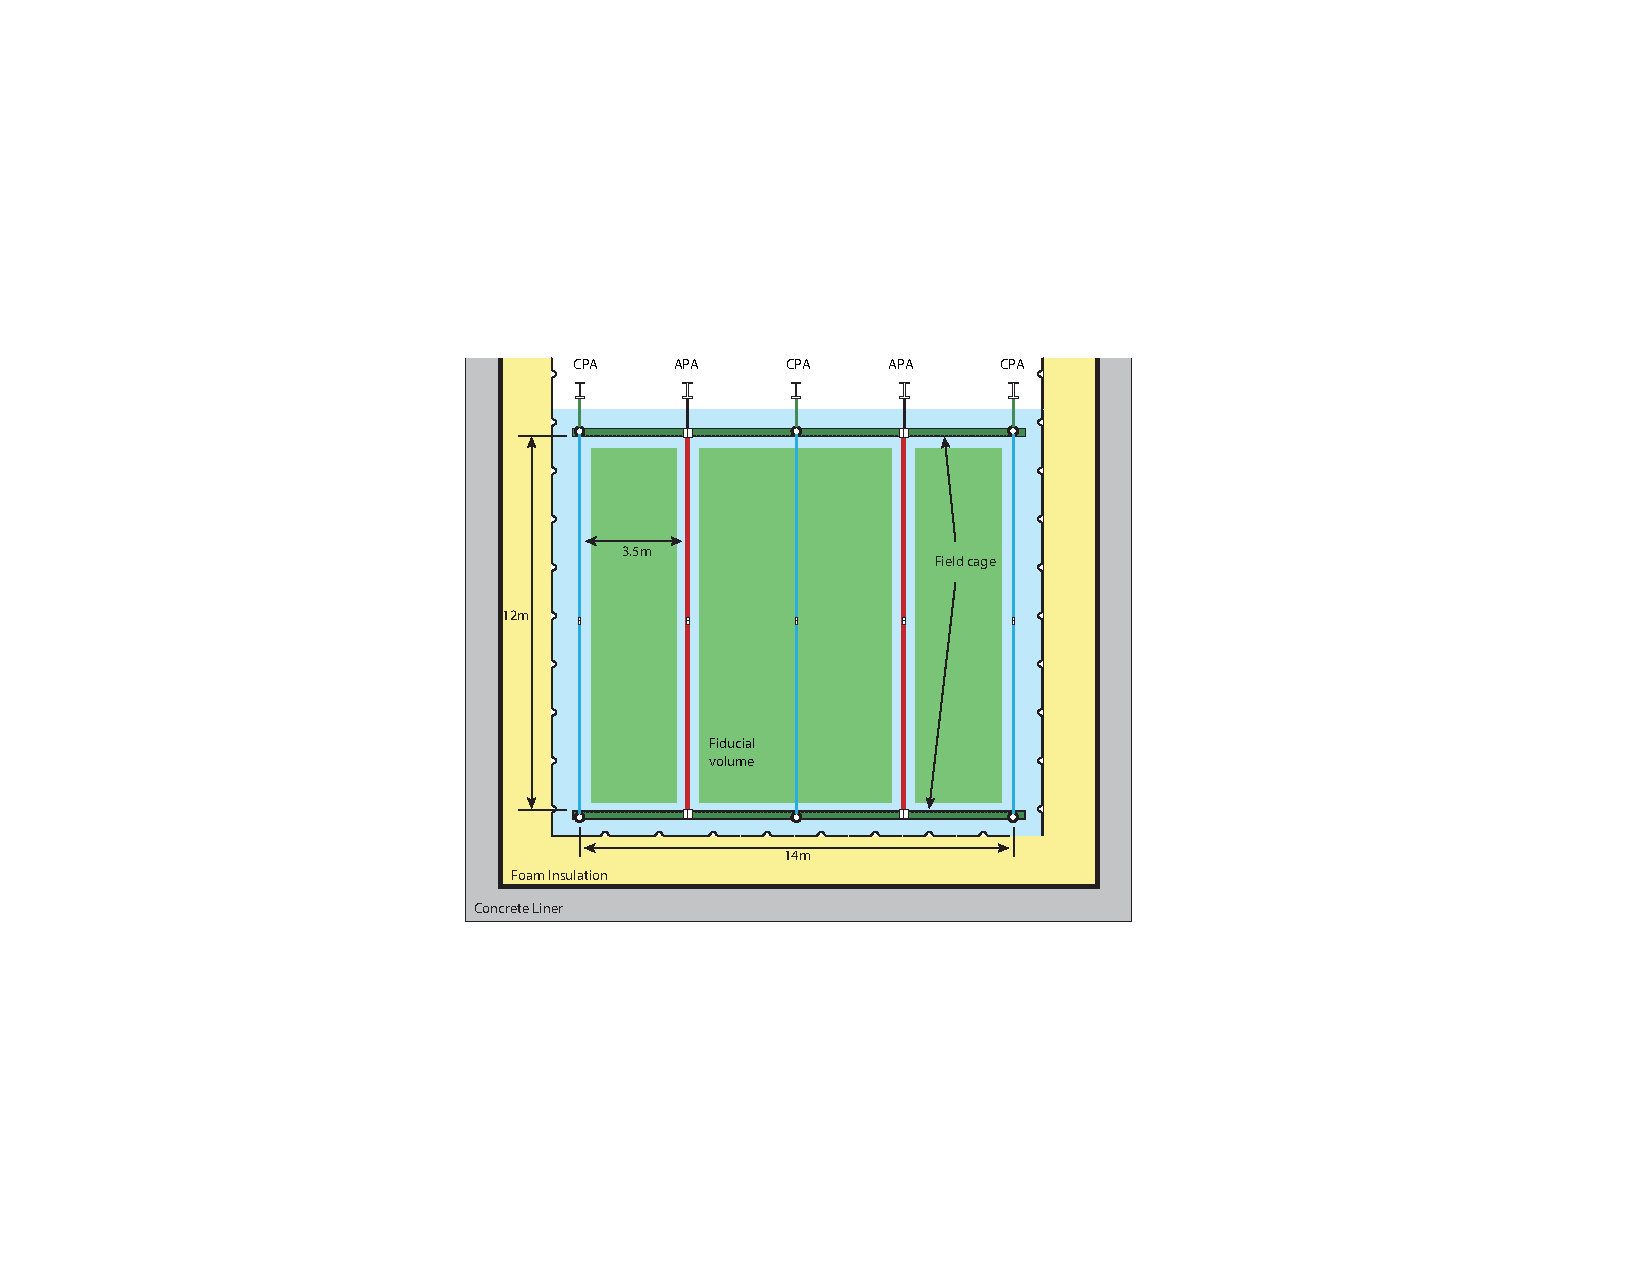
\includegraphics[width=\linewidth]{ELBNF_FD_Cross_Section.pdf}
\caption[Cross section of the TPC inside the cryostat]{Cross section of the 5 kton fiducial mass TPC inside the cryostat.  The length of the TPC is  30~m along the direction of the neutrino beam (into the paper). }
\label{fig:tpc-xsect1}
\end{figure}

The TPC's active volume (Figure~\ref{fig:tpc-xsect1}) is 12~m high, 14~m wide and 30~m long in the beam direction. 
Its three rows of CPA planes interleaved with two rows of APA planes 
are oriented vertically, parallel to the beamline with the  
electric field applied perpendicular to the planes.
The maximum electron-drift distance between a cathode and an adjacent 
anode is 3.4~m. The anode plane assemblies are 
2.3~m wide and 6~m high. Two 6-m modules stack vertically to 
instrument the 12~m active depth. In each row, 13~such stacks are placed 
edge-to-edge 
along the beam direction, forming the 30~m active length of the detector.  Each CPA has the same width, but half the height ($\sim$3~m) as an APA for ease of assembly and transportation.  4 CPAs will be stacked vertically to form the full 12~m active height. 
Each cryostat houses a total of 52~APAs and 156~CPAs.
Each facing pair of cathode and anode rows are surrounded by a 
``field cage,'' assembled from panels of FR-4 sheets with parallel copper strips connected to resistive divider networks. 

On each APA, four planes of wires cover each side of a frame (the ``wire frame''). See Figure~\ref{fig:tpc-wire-frame-xsect}.
The inner three planes of wires are oriented, going from the inside out: vertically, and at $\sim\pm$36$^\circ$ 
to the vertical, respectively. Each wire is connected to a front-end readout channel.
The wires on the outermost plane are oriented vertically, and are not connected to the readout electronics.
At a nominal wire pitch (center-to-center separation) of 4.8~mm,
the total number of readout channels in an APA is 2560, for a total of 133,120 in each cryostat.
 
As shown in Fig.~{\ref:tpc-wire-frame-xsect}, the readout electronics reside only along one narrow edge of an APA. During installation, 2 APAs are interconnected on their non-readout ends, leaving the readout ends completely outside of the TPC's active volume.  Cables from the bottom APAs can either routed through the hollow vertical APA frames, or down along the floor and up along a side wall of the cryostat.

\begin{figure}[htpb]
\centering
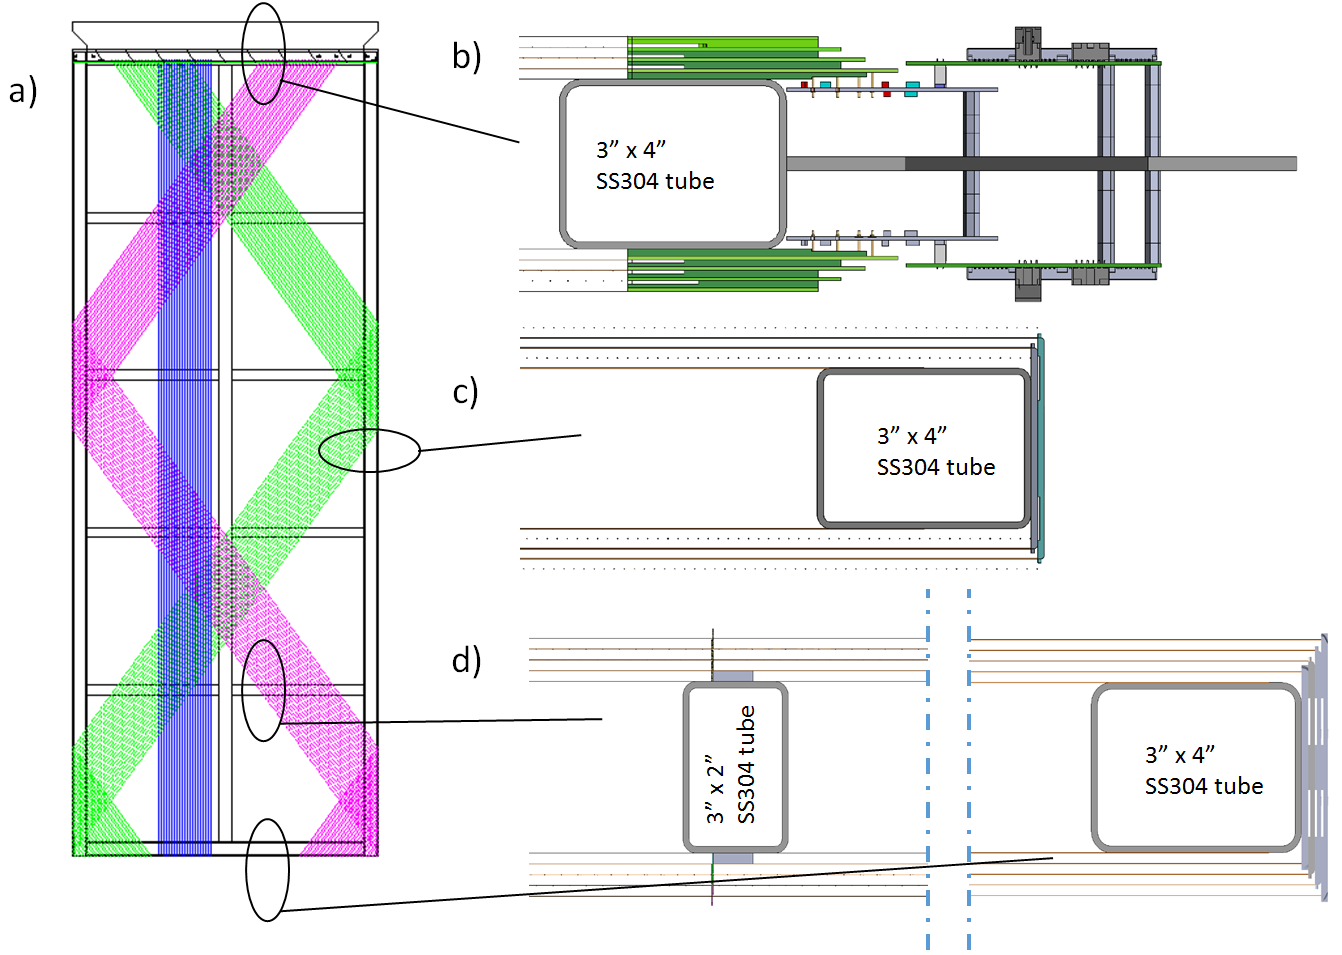
\includegraphics[width=\linewidth]{tpc_apa_cross_sections}
\caption[Illustration of the APA wire wrapping scheme]{Illustration of the APA wire wrapping scheme, and three cross sectional views. } 
\label{fig:tpc-wire-frame-xsect}
\end{figure}

%%%%%%%%%%%%%%%%%%%%%%%%%%%%%%%%
\section{Design Considerations} 
\label{sec:v5-tpc-reqs-n-specs}

The requirements for the TPC can be found in the requirements documentation \cite{lar-fd-req}. The most significant ones are the following:

\begin{itemize}	
\item Provide the means to detect charged particles in the detector and transmit the detector signals to the Data Acquisition System (DAQ)
\item Meet the physics requirement for electron/photon discrimination;  the TPC wire spacing will be $<$~5~mm
\item Limit variation in the wire sag to $<$ 0.5~mm such that it does not significantly impact the position and energy resolution of the detector
\item Provide redundancy in the discrimination of electrons from photon conversions and ensure long-term reliability over the life of the experiment;  configuration will use three instrumented wire planes
\item Optimize the measurement of high-energy and low-energy tracks from accelerator-neutrino interactions; the wire-plane orientation is optimized for neutrinos in the LBNE energy range
\item Enable the detector to distinguish a Minimum Ionizing Particle (MIP) from noise with a signal-to-noise ratio $>$ 9:1
\item Enable the detector to measure the ionization up to 15 times that of a MIP particle; this is necessary to perform particle identification of stopping kaons from proton decay
\item Enable the in-vessel electronics to operate for the life of the facility
\item Record the wire-signal waveforms continuously without dead time
\item Use only materials that are compatible with high-purity liquid argon

\end{itemize}

The TPC is comprised of several interconnected subsystems – APAs, CPAs, Field Cage, and High Voltage Feed-throughs. A system engineering design and development approach will be taken to ensure that the various subsystems are properly integrated and the system is designed end-to-end to meet performance requirements. This approach will be led by a system engineer that will ensure that interfaces are defined and managed, that requirements for each subsystem and the TPC as a whole are defined and understood, analyses are performed where needed, prototyping is performed to retire or mitigate risk, and that test plans meet verification and validation requirements. The most significant challenge for the TPC is the LAr cryogenic environment. The TPC architecture will handle the cryogenic thermal cycles, accommodate the cryostat roof motion, and mitigate potential microphonics noise generated by wire vibrations.

The design approach will take inputs from several sources.  These sources include requirements from the scientific collaboration to ensure integrity of the physics data, studies of what has been successful in smaller scale TPC's, sharing of knowledge, ideas, and concepts with others in the LAr TPC community, and analysis and evaluation of the performance of the 35ton prototype.  These inputs will be distilled into functional requirements.  These functional requirements will be used to define alternative concepts or architectures for the TPC.  These concepts will drive preliminary requirements for the TPC interface with the cryostat and the conventional facilities.  They will also be used to define the preliminary interface requirements between the structural components and the modular subassemblies of the TPC.  These alternate concepts will be tested and analyzed as needed and reviewed with the physicists, conventional facilities, the cryostat manufacturer, and TPC engineers.  Based on analysis and feedback, the preferred concept will be further developed and detailed into final requirements and specifications for the physical internal and external interfaces.  These requirements and specifications will be clearly communicated to the responsible engineering groups.


%%%%%%%%%%%%%%%%%%%%%%%%%%%%%%%%
\section{Anode Plane Assemblies}
\label{subsec:v5-tpc-chamber-apa}

The APAs are 2.3~m wide, 6.3~m long, and 12~cm thick. The length is chosen for fabrication purposes and compatibility with underground transport limitations. The 2.3-m width is set to fit in a standard HiCube container for storage and transport with sufficient shock absorbers and clearances. 
Each APA is constructed from a framework of light-weight, stainless-steel rectangular tubing, with four layers of wires wrapped over both sides of the frame. The front-end electronics boards are mounted on one end of the wire frame and protected by a metal enclosure.  

%%%%%%%%%%%%%%%%
\subsection{Wires}

The wires used in the TPC must provide:
\begin{itemize}
\item High break load to withstand the applied tension 
\item Good conductivity to minimize noise contribution to the front-end electronics
\item Comparable thermal-expansion coefficient to that of the stainless-steel 
frame to avoid tension change after cool-down
\end{itemize}

Both stainless-steel and copper-beryllium (CuBe) wires are potential candidates.  
Stainless steel was the choice of ICARUS, while a copper-plated 
stainless-steel wire was chosen by MicroBooNE  (to reduce resistance).  Both experiments use a wire-termination 
technique that is labor-intensive and impractical for LAr-FD. Previous experience from FNAL \cite{FNAL-proto-APA} has shown that a CuBe wire under 
tension can be reliably bonded to a copper-clad G10/FR4 (glass epoxy material) surface by a combination of  epoxy (mechanical bonding) 
and solder (electrical connection).  This bonding technique greatly simplifies the electrical 
connection to the readout electronics and it can be easily automated 
with commercial equipment.  Therefore CuBe wire is 
selected as the reference design wire of choice.

At 150~$\mu$m diameter,  the breaking tension of a hardened CuBe wire is $\sim$30~N.  
To ensure no wire breakage in the TPC, e.g. during cryostat cool-down, the nominal operating tension of the wire will be set at 5~N.  Periodic support structures on the wire frame will
limit the unsupported wire length to less than 1.5~m, resulting in less than 0.2~mm deflection due to gravitational or electrostatic forces.  Wire ends will be glued and soldered (if electrical connection is needed) 
onto printed circuit boards attached to the wire frame.

\begin{figure}[htbp]
\centering
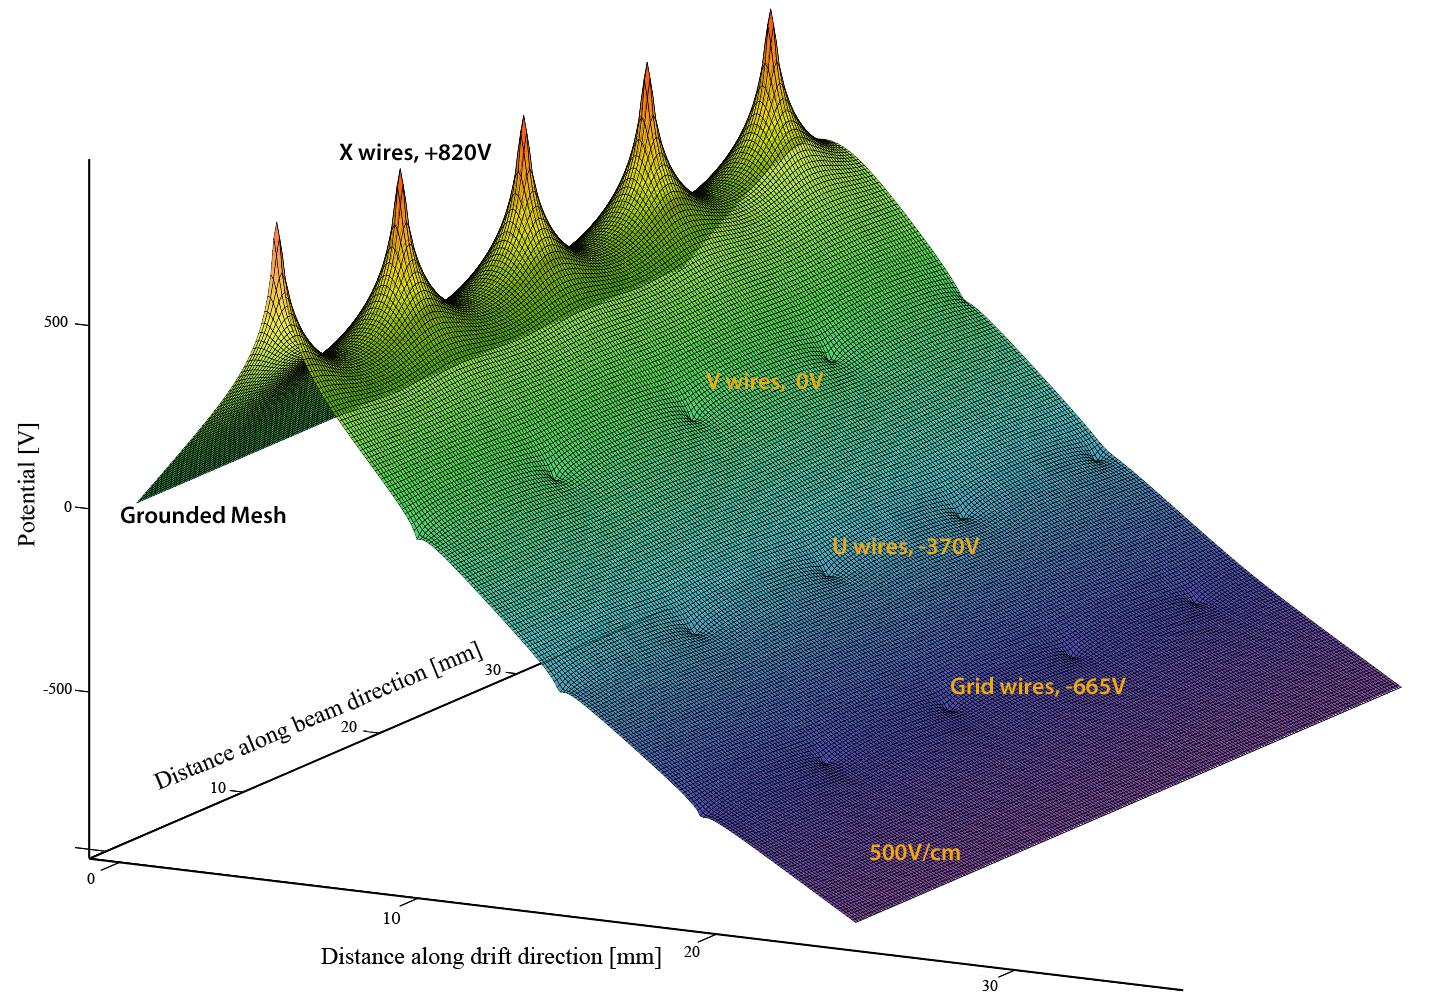
\includegraphics[width=\linewidth]{v5c3-bias-voltages.png}
\caption[Plot of electric potential distribution near the wire planes]{A surface plot of the electric potential distribution near the wire planes.  The voltages on the wire planes are biased to provide complete electron transparency through the first three planes, and complete collection on the fourth plane. }
\label{fig:tpc-bias-voltages}
\end{figure}

%%%%%%%%%%%%%%%%
\subsection{Wire Planes}


Four planes of wires are installed on each side of an APA as shown in Figure~\ref{fig:tpc-wire-frame-xsect}.
A nominal wire pitch of 4.7~mm is selected to meet the position resolution  and signal-to-noise ratio requirement. The distance between wire planes is set to 4.8~mm (3/16~in) to use standard printed circuit board thickness, while maintaining optimal signal formation.  These four planes (along the direction of electron drift) are labeled as: the {\em grid plane}, the {\em first induction plane} (U), the {\em second induction plane} (V), and the {\em collection plane} (X).
The wires on the grid and the collection planes
are vertically oriented, while the two induction planes are oriented 
at $\sim\pm$35.71$^\circ$ to the vertical. This wire layout is shown to be very good for reconstructing beam-neutrino events \cite{wire-orientation}. The wires on the grid plane are not 
connected to the readout electronics; they shield the first induction wire plane from being influenced by distant arriving ionizations. The four wire planes 
will be electrically biased so that electrons from an ionizing-particle
track completely drift past the first three planes and are collected by the 
fourth plane. Calculations show that the minimum bias voltages 
needed to achieve this goal are $V_G= -665$V, $V_U=-370$V, $V_V=0$V and $V_X=820$V 
respectively.  A grounded mesh plane, located 4.8~mm behind the collection plane, prevents the electric field around this set of wires from being distorted by the metal frame structure and the wires on the opposite side of the frame. It also shields the sensing wires from potential EM interferences from the silicon photomultipliers (SiPMs), discussed in Chapter~\ref{ch:photon}, mounted within the frame.  The mesh should be have a wire pitch less than 2~mm to ensure a uniform electric field and a high optical transparency.  Figure~\ref{fig:tpc-bias-voltages} shows the electric potential distribution near the APA frame with the wire planes biased with the appropriate voltages. 

The V wire plane is directly connected to the front-end electronics, i.e. $V_V=0$V, to simplify the coupling and 
reduce the maximum bias voltages on the other planes. The wires on the two induction planes (U \& V) are wrapped in a helical pattern around the long edges of the wire frame 
(Fig.\ref{fig:tpc-wire-frame-xsect}a). This technique makes it possible to place readout 
electronics only at one short edge of a wire frame, enabling joining the APAs on the other three sides with minimal dead space.  It slightly complicates 
the track reconstruction because the U \& V wires are sensitive to tracks on 
both sides of the APA.  The upper APAs in the cryostat will have their readouts
at the top edge of the frame (as shown in Figure~\ref{fig:tpc-wire-frame-xsect}), 
while the lower APAs will mount their electronics at the bottom edge.  These readout electronics are located outside of the TPC's active volume.

The wire angle and overall APA length are chosen so that the angled wires wrap less than one full wrap around the APA between its head and foot (Fig.~\ref{fig:tpc-wire-angle}).  This avoids an ambiguity problem that would arise if a pair of angled wires and a vertical wire coincided at more than one location on an APA face.  A particle arriving at one of the locations would be indistinguishable from a particle arriving at the other.  The multiple photon detectors embedded in the APA frame also help to identify the vertical location of an ionizing track.

\begin{figure}[htbp]
\centering
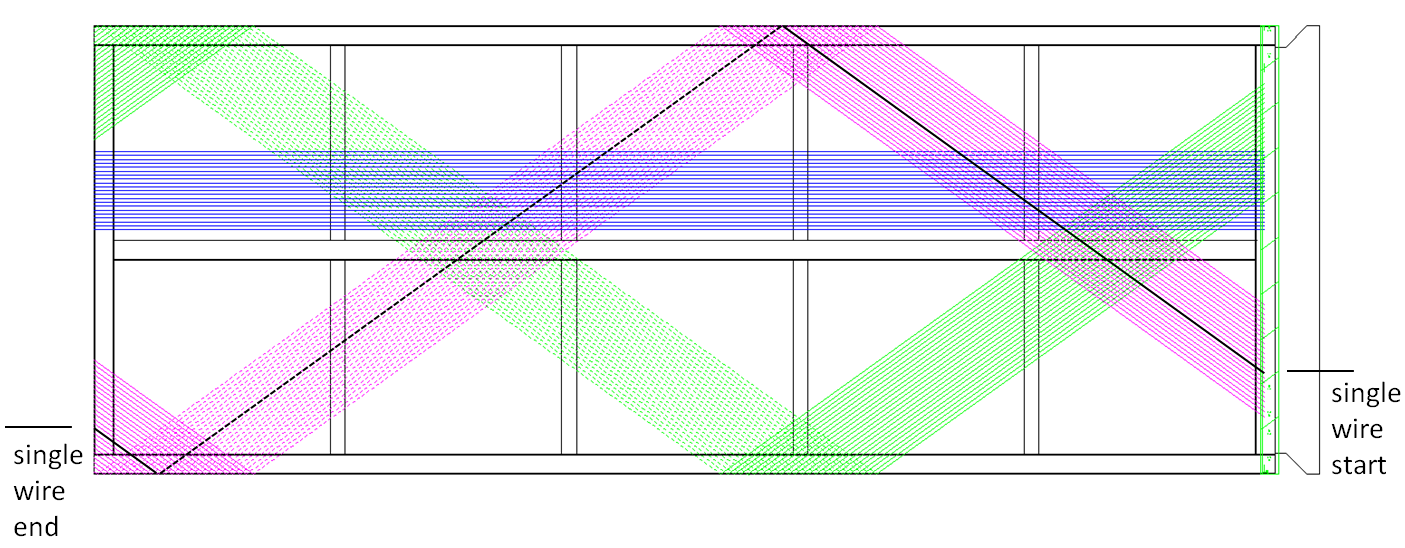
\includegraphics[width=\linewidth]{tpc_apa_wire_wrapping.png}
\caption[TPC APA wire wrapping illustration]{An illustration of a few wire paths on the APA.  The length and width of the APA, and the wire angle, are chosen so that in the angled layers the wires wrap less than once around the APA.  This can be seen in the darkened path of a single wire in the illustration.  Small portions of the wires from the three signal planes are shown in color.  There is a fourth, un-shown wire plane above these three which is present to help maintain a uniform field and shield the induction planes from interference. }
\label{fig:tpc-wire-angle}
\end{figure}


Precise values of wire angle and wire pitch were chosen to give an integral number of wires across the boards at the electronics end of the APA as well as an integral number of wire slots in the boards along the sides of the APA.  A solder pad spacing at the electronics end of 5.75~mm and a wire slot spacing along the sides of 8.00~mm results in a wire to wire pitch of $\sim$4.67~mm and a wire angle of 35.71$^\circ$ to the long axis of the APA.


The 5.75~mm pitch of solder pads across the electronics boards of the U and V layers results in 40 channels per 230~mm wide board.  The $\sim$4.79~mm pitch in the X layer gives 48 channels per 230~mm wide board.  Each 230mm wide stack of boards has, therefore, 40+40+48=128 channels.  There are 10 of these board distributed per side along the readout edge of an APA for a total of 2560 signal wires on the APA.  With the additional 48 G wires per board stack, the total number of wires per APA is 3520.




\begin{figure}[htpb]
\centering
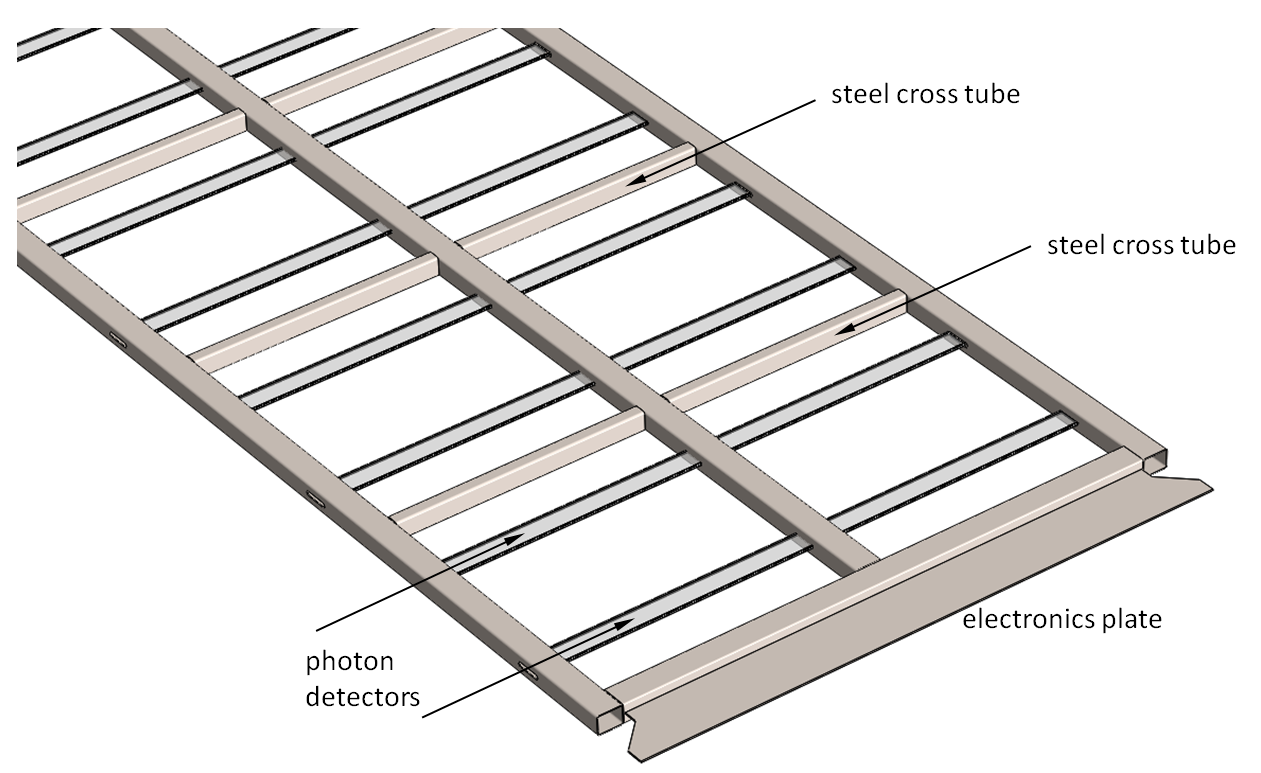
\includegraphics[width=\linewidth]{tpc_apa_frame.png}
\caption[Conceptual design of a wire frame]{The stainless steel APA frame (shown without wires or boards). The photon detectors are shown in place – although the APA is designed so that the photon detectors can be inserted into the APA after the wires are wound. }
\label{fig:tpc-wire-frame}
\end{figure}

%%%%%%%%%%%%%%%%
\subsection{APA Frame}

At a nominal wire tension of 5~N, the 3520 wires exert a force of 
$\sim 7.0$~kN/m on the short edges of the APA, and a 
$\sim 1.5 $~kN/m force on the long edges. The wire 
frame must be able to withstand the wire tension with a minimal 
distortion, while minimizing the thickness of the 
frame to reduce the resulting dead space. A conceptual design 
of the wire frame is shown in Figure~\ref{fig:tpc-wire-frame}.  
It is constructed from all stainless-steel tubes welded in a jig.  
Structural analysis has shown that the maximum distortion of the frame due to wire tension is less than 0.5~mm. The total mass of a bare frame is $\sim$260~kg.

Lengthwise buckling is not an issue, both because of the strength of the frame and because the wires are maintained at an approximately uniform distance from the frame by periodic comb-like structures (Fig.~\ref{fig:tpc-wire-support}).

All three long tubes have slots cut in them so the photon detectors can be inserted into the APAs after the wires are installed.  The two long outer members of the frame are open-ended, so the photon detector cables can be threaded through them.  All tube sections are vented to prevent the creation of trapped volumes.



%%%%%%%%%%%%%%%%
\subsection{Wire Wrapping Around an APA}


\begin{figure}[htpb]
\centering
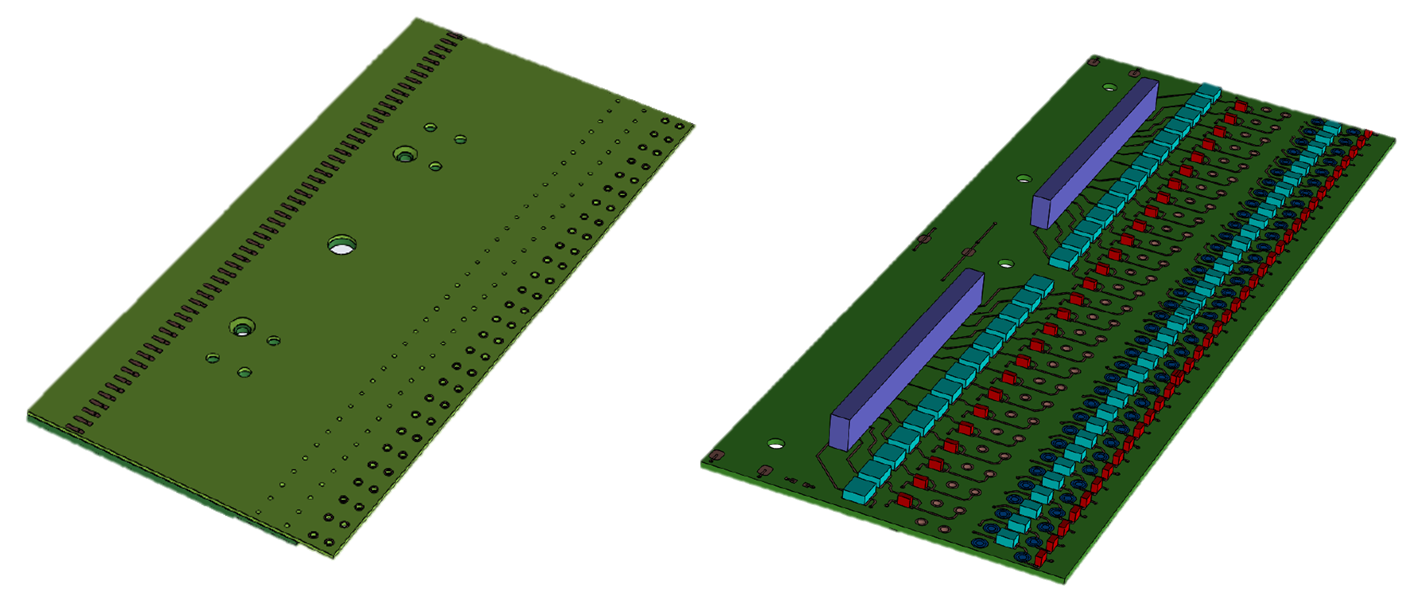
\includegraphics[width=\linewidth]{tpc_apa_x_cr_boards.png}
\caption[Conceptual design of a wire bonding board for the x wires]{Left: Design of a wire bonding board for the x wires.  The wires are glued on the leading edge of the top surface, and then soldered to the soldering pads. Right: Another board, located underneath the four wire boards, carries the RC network for the bias voltages. }
\label{fig:tpc-wire-board-x}
\end{figure}



The wire boards are the interface between the wires and the data acquisition electronics.  Also, they physically anchor the wires at the top end of the APA.  The four planes of wires are attached to their respective wire boards through a combination of epoxy and solder. During winding of the X layer onto the APA the wires are placed across the top surface of the X wire board. The wires are then glued down with a strip of epoxy at the leading edge of the board.  After the epoxy has cured, the wires are soldered onto the copper pads under each wire, and then the wires are cut beyond the pads. The V, U and G planes are attached on top of the X boards and similarly populated with wires, one layer at a time. An array of pins is pushed through holes in the stack of wire boards, making electrical connections between the wires and the CR board.   
Figure~\ref{fig:tpc-wire-board-x} shows one of the X boards and an intermediate board, the capacitor-resistor (or CR) board, which is located between the wire boards and the front end electronics boards.  

In this way the wire board are connected to the bias voltage supply through the resistor-capacitor network on the CR board. The resistors in this network have values around 20 M$\Omega$, so that in the event that a wire from a different plane breaks and is shorted to these wires, the bias voltages on the rest of the wires will not be affected. The AC-coupled signals from the RC network are connected to sockets that will mate with the front-end readout boards.

These readout boards, as described in Section ?, process the analog signals from the wires and transmit the digital information via feedthroughs to the DAQ system outside the cryostat. The electronics on the readout boards generate an estimated 60 W of heat per APA which may produce a small quantity of argon bubbles.  Stainless-steel covers are placed over the readout boards to contain the bubbles and direct them to the gas volume of the cryostat. In the case of the lower APAs, the bubbles, if not already re-condensed, will be funneled through the vertical hollow frame members to the top of the cryostat.


Figure \ref{fig:tpc-APA-corner} is a close-up view of a corner of an APA frame with some wires and various wire boards to demonstrate the assembly.

After the grid plane wires are placed on the APA, and fiberglass cover sheets placed over the edge boards, metal guards are placed along the three wrapped edges of an APA. These guards protect the fragile wires during APA handling, storage and transport.



\begin{figure}[htpb]
\centering
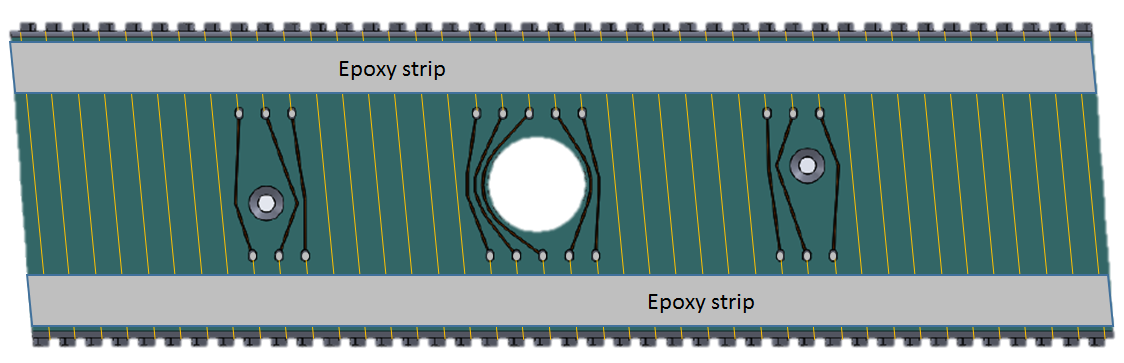
\includegraphics[width=\linewidth]{tpc_apa_u_edge_board}
\caption{Design of a wire wrapping board for the U wires on a long edge of an APA. The light, angled lines represent the wires wrapped over the board surface. Some wires near the mounting holes must be soldered to the copper traces and then cut.  An epoxy strip attaches the wires to the board so the solder is only critical for the electrical connection.}
\label{fig:tpc-wire-board-u-side}
\end{figure}

\begin{figure}[htbp]
\centering
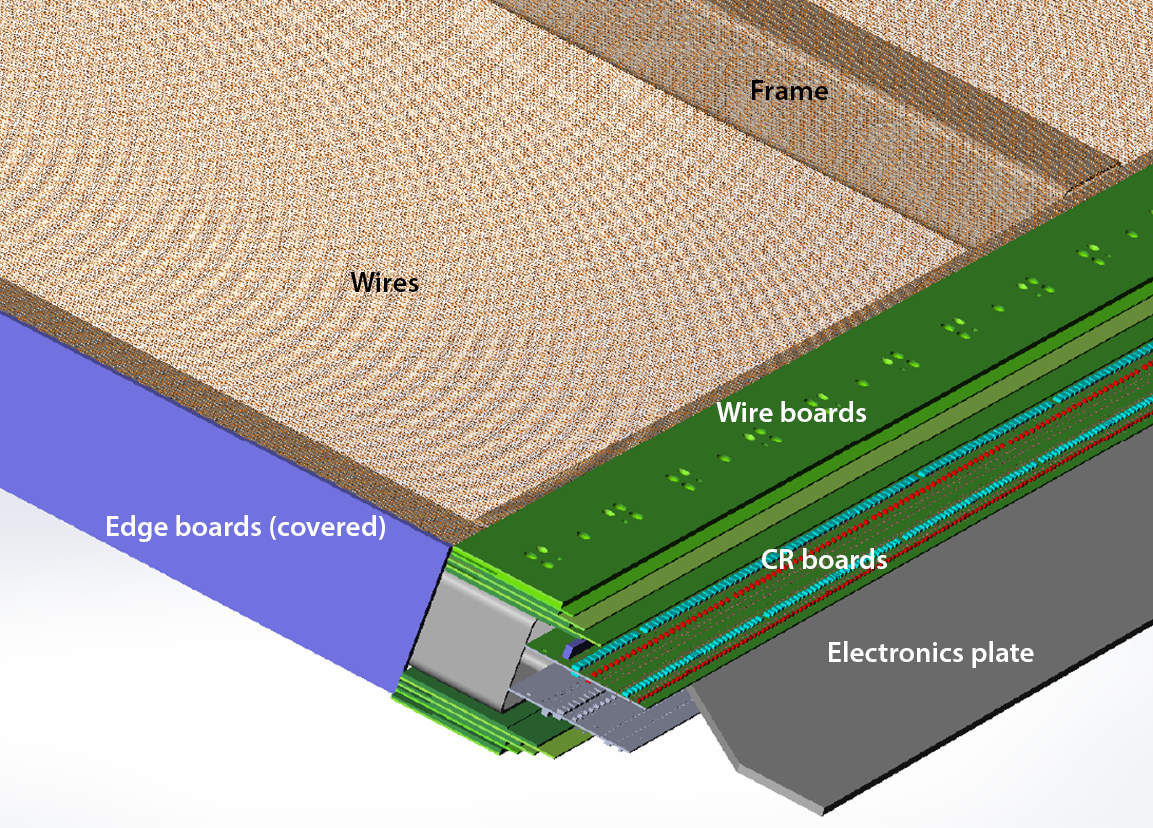
\includegraphics[width=\linewidth]{tpc_apa_module_corner.png}
\caption[Closeup view of a partially assembled corner of an APA]{A close-up view of a partially assembled corner of an APA.  The wire boards and CR boards are shown but the ``cold electronics boards'', for data acquisition, are not shown.  They mount on the electronics plate and connect electrically to the CR boards. }
\label{fig:tpc-APA-corner}
\end{figure}

%%%%%%%%%%%%%%%%
\subsection{Wire Supports on Inner Frame Members}

Figure \ref{fig:tpc-wire-support} shows the comb set that provide intermediate support to the long wires.  Combs are located on each of the 4 cross beams so that the longitudinal wires are supported every 1.2m and the angled wires about every 1.5m while introducing only millimeter-scale dead regions.

The support structure is composed of strips of thin G10 sheet, with notches machined at correct intervals. The support strips for the X plane are mounted on the surface of the cross tubes.  After all X wires have been placed into the slits, the V support strip (shown in green) is glued onto the tips of the X strips, trapping the X wires in position.  After the V wire are placed into the slits, the U support strip (identical to the V strip) is glued to the V strip, trapping the V wires.  These wire supports play a key role in minimizing wire deflection due to gravity and electrostatic force, enabling the use of a moderate wire tension and reducing the risk of wire breakage.



\begin{figure}[htpb]
\centering
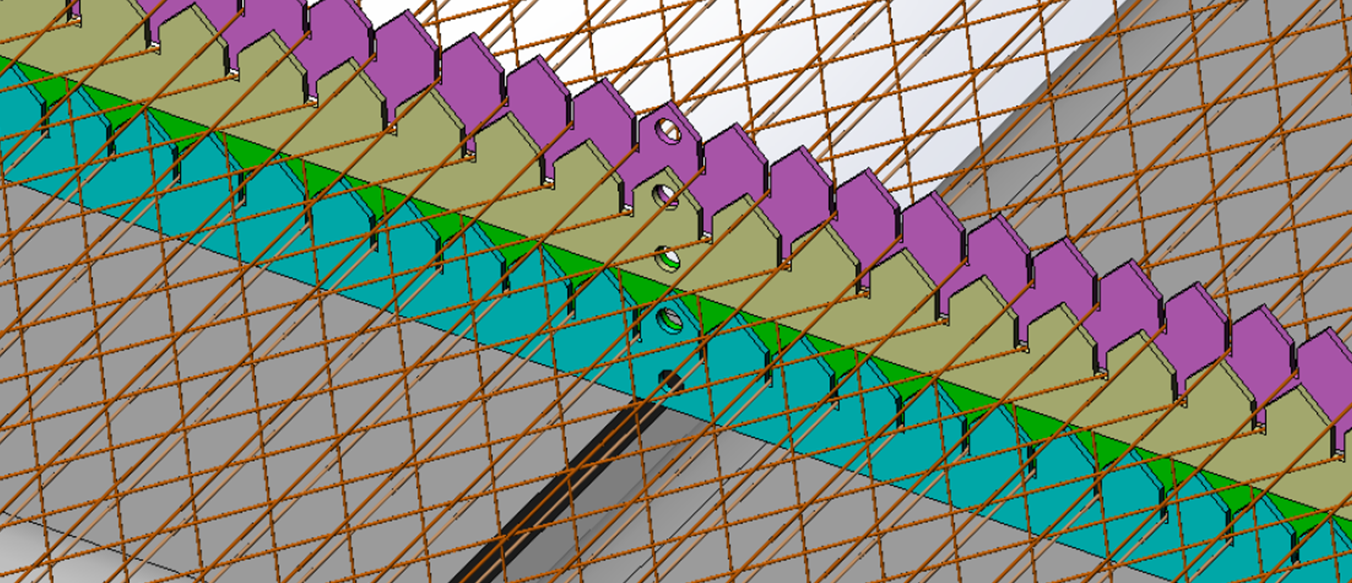
\includegraphics[width=\linewidth]{tpc_apa_wire_support.png}
\caption[Conceptual design of the wire support for the U, V \& X wires]{Intermediate wire support combs.  A set of thin G10 combs is located on each cross bar of the frame.  Each layer of wire has its own comb and, as each new comb is glued to the previous one, it locks in the previous layer of wire.  In this view the tips of the second layer (green) combs are hidden behind the body of the third layer (tan) combs.  One more retainer strip would be added to the above combs to hold the top wire layer in place.  The row of holes in the comb are used with a registration/alignment fixture.}
\label{fig:tpc-wire-support}
\end{figure}

\begin{figure}[htpb]
\centering
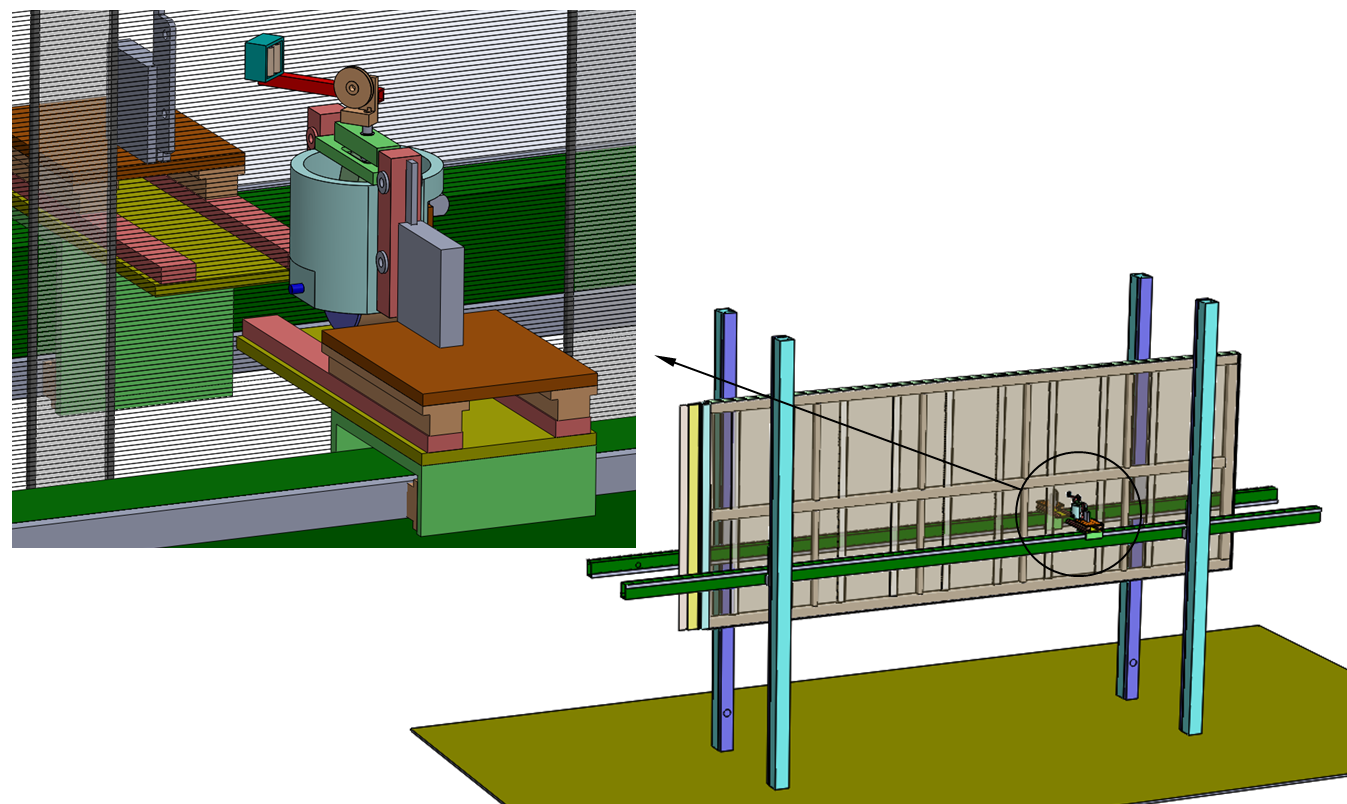
\includegraphics[width=\linewidth]{tpc_apa_winding_machine.png}
\caption[Winding machine concepts]{The tensioner head is passed from one side of the APA to the other as it’s moved around the APA to wind wire onto the APA frame.  The horizontal/vertical positioning systems on each side of the APA are made of commercial linear motion components.  Much or all of the positioning systems should be available from commercial vendors}
\label{fig:tpc-winding-machine}
\end{figure}

%%%%%%%%%%%%%%%%
\subsection{Wire-Winding Machines}

A winding machine will be constructed to lay the 3520 wires onto each APA. It has sufficient versatility that the same mechanism can wind both the angled and the longitudinal layers.  This was not a deliberate goal in the beginning but it has turned out that the method chosen for winding the angled layers will work for the longitudinal layers as well.
 
Its working concepts are illustrated in Figure~\ref{fig:tpc-winding-machine}. 
The wire tensioner is a self-contained unit that includes the wire spool.  It is designed so that tension is maintained, not just when wire is pulled out, but also if wire is let back into the tensioner.  The APA is held off the ground by a couple posts, with one of its long edges down.  There are X-Y positioners on either side of the APA; the tensioner is moved across the face of the APA by one of these positioners – unspooling tensioned wire as it moves.  When the tensioner arrives at the edge of the APA it is passed across to the positioner on the other side of APA.  This is done in the correct position so that wire is placed into the appropriate slots of the edge boards. The new positioner then moves it to the next location on the edge - where it is passed back around the edge of the APA.  In this way the entire layer of wire can be placed on the frame.  There will be a couple supports on the long side of the APA nearest the floor and one or two on the long side at the top.  At some point in the winding of the angled layers, the machine will have to be stopped and the supports moved out of the way -- to locations that have already been covered with wire.

Although a large part of an entire plane of wires can be wound in one continuous process, a more fault-tolerant procedure would be to pause the winding machine periodically and solder the last wire. This intermediate soldering step will prevent the unwinding of a large section due to an accidental broken wire.  An automatic soldering robot will solder the wire ends after the wires have been laid down on the APA. A wire-tension measuring device will scan the newly placed wires and record the wire tension of each wire. Any wires with abnormal tension will be replaced manually.



%%%%%%%%%%%%%%%%%%%%%%%%%%%%%%%%
\section{Cathode Plane Assemblies}
\label{subsec:v5-tpc-chamber-cathode}

\begin{figure}[t]
\centering
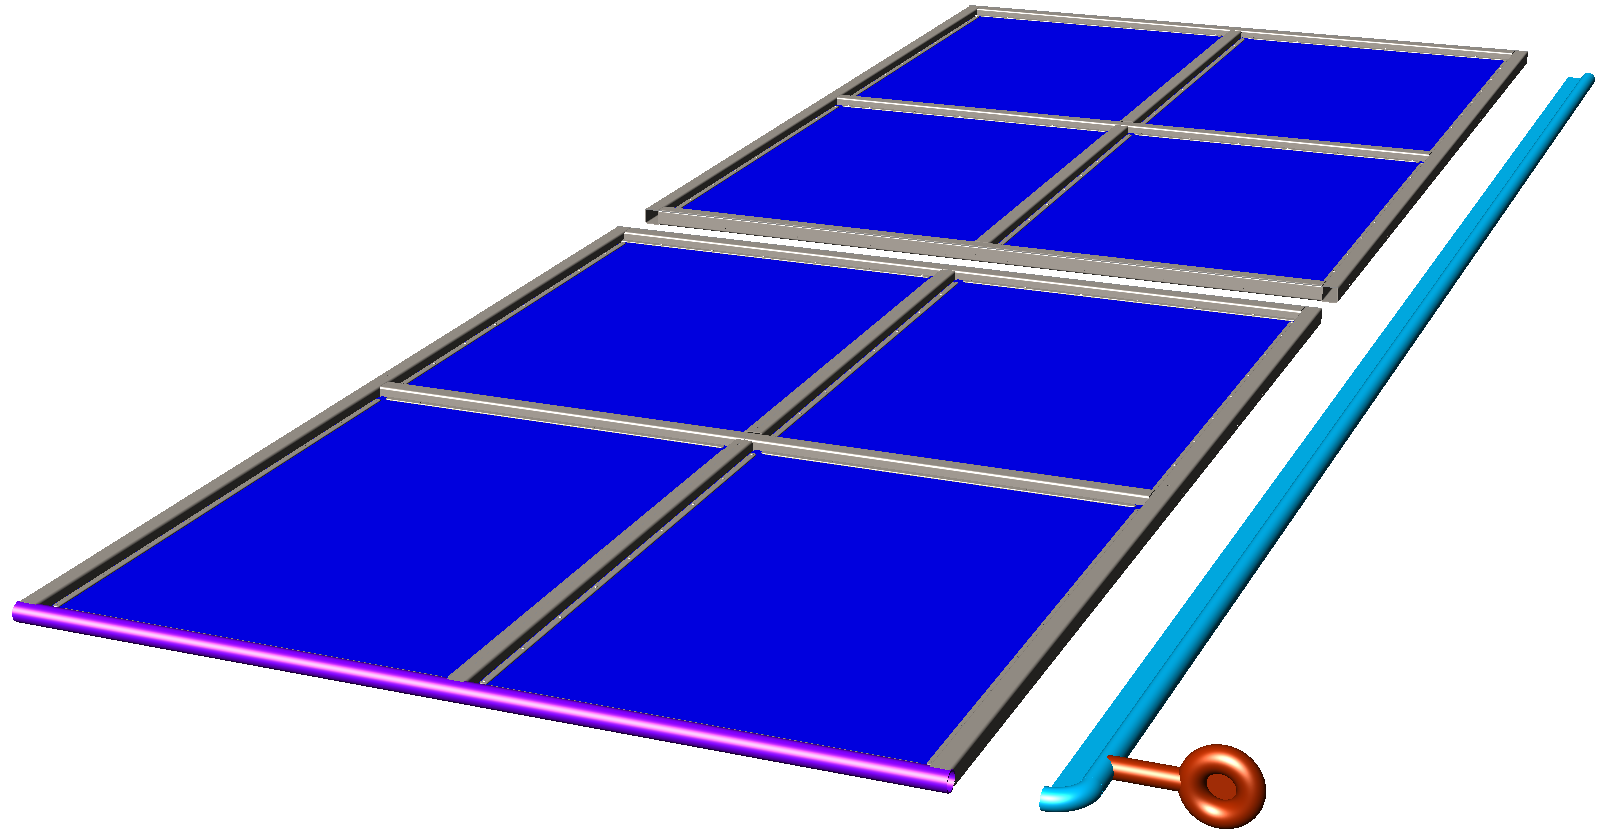
\includegraphics[width=\linewidth]{tpc_cpa_components}
\caption[Conceptual design of the cathode plane assembly]{Conceptual design of the different cathode plane components near a corner of a cathode wall.  Two flavors of CPAs (edge unit and non-edge unit) make up the entire wall of a cathode plane, terminated at both ends by the end pieces (cyan colored).  A high voltage receptacle (orange) connects with the HV feedthrough from the cryostat ceiling. Each CPA is roughly 2.3m wide by 3m tall. }
\label{fig:tpc-cathode-model}
\end{figure}


There are 3 walls of cathodes in each TPC.  Each wall is tiled from a 4 unit high by 13 unit wide array of cathode plane assemblies (CPAs). Figure~\ref{fig:tpc-cathode-model} shows a corner of a cathode plane.  Each CPA is 2.3~m wide (identical to the APA width) and 3~m tall (half of APA height) for ease of fabrication, assembly and handling.  Each CPA is made of a stainless-steel framework, 
with panels of solid stainless steel sheets mounted between the from openings.  Along each vertical  columns of the 4 CPAs, there are two slightly different versions: the edge CPAs (top and bottom rows ), and the non-edge CPAs (2nd and 3rd rows).  The non-edge CPAs use all square tubes for the frame structure, while the edger CPAs uses a round tube on the outside edge of the CPA facing the floor or ceiling of the cryostat to minimize the surface electric field.  Two sets of field shaping end pieces are installed at the two ends of the CPA wall to properly terminate the cathode wall with rounded edges.  All CPAs are suspended from the ceiling using G10 hangers to insulate the CPA from the cryostat.


The impact of the square tube frame on the drift field near the cathode will be evaluated in the 35ton TPC study.  If necessary, we can attach strips of field shaping electrodes with a suitable bias voltage on the raised square tube surfaces to correct the field distortions.  


This CPA design forms a highly conductive wall at $-$170~kV facing the grounded cryostat wall with a $\sim$ 0.6~m clearance.  As a results, the stored energy on this cathode is more than 100~joules.  There is a risk of damage to the cryostat membrane or other TPC components if a high voltage discharge develops, and dumps all the energy quickly at a very small surface area. To mitigate this risk, we are currently analyze the electrical properties of the cathode, and developing cathode designs that will substantially slowdown the total energy release in case of a discharge.  Possible choices include a highly resistive coating on all non-conductive cathode surface panels as well inner frame members; or conductive panels with robust resistive coupling to the frame structures.




%%%%%%%%%%%%%%%%%%%%%%%%%%%%%%%%
\section{Field Cage}
\label{subsec:v5-tpc-chamber-fieldcage}

Each pair of facing cathode and anode rows forms an electron-drift region. A field cage  completely surrounds the four open sides of this region
to provide the necessary boundary conditions to ensure a uniform electric field within, unaffected by the presence of the cryostat walls.

\begin{figure}[htbp]
\centering
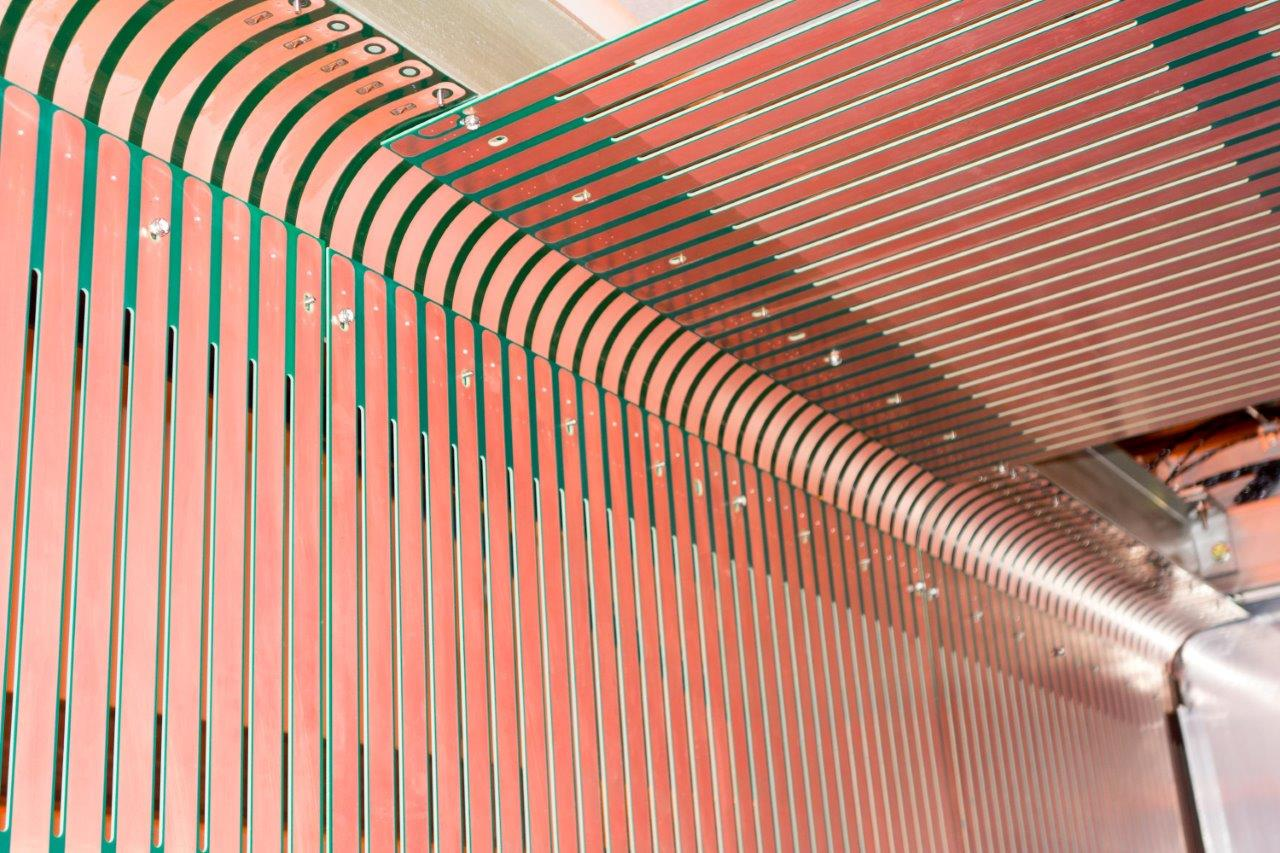
\includegraphics[width=4in]{tpc_fca_35t.jpg}
\caption[35ton field cage]{A corner of the 35ton TPC field cage as it is being constructed. }
\label{fig:tpc-field-cage}
\end{figure}    

The entire TPC requires $\sim 1100 \rm{m}^2$ of field 
cage material per 5-kton detector. The field cages are constructed using copper-clad FR4 sheets reinforced with fiber glass I-beams to form panels of 2.3~m $\times$ 3.4~m in size. Parallel copper strips are etched/machined
on the FR4 sheets. Strips are 
biased at appropriate voltages provided by a resistive-divider network. These strips will create
a linear electric-potential gradient in the LAr, ensuring a uniform drift 
field in the TPC's active volume.  Simulations have shown that the drift-field non-uniformity quickly drops below 1\%, roughly 
a strip pitch away from the field-cage surface. 

Since the field cage completely encloses the TPC drift region on four sides, while the solid cathodes blocks the remaining two, the FR4 sheets must 
be frequently perforated to allow natural convection of the liquid argon.  
The ``transparency'' of the perforation will be determined by a 
detailed LAr computerized fluid dynamic (CFD) study.


The resistor-divider network will be soldered directly onto the field-cage panels. 
Multiple resistors will be connected in parallel between any two taps of the divider,
in order to provide fault tolerance. 
One end of the divider chain is connected directly to the cathode, while the other end is connected to ground at the APA through resistors of the appropriate value. 
In additional to the resistor network, surge suppressors such as varistors and gas discharge tubes will be installed between each field cage strips to avoid an over-voltage condition that occurs between field cage electrodes and the cathode in a high voltage discharge.


The major challenge of this field cage design is to minimize the electric field exposed to the liquid argon near the thin copper strips.  One solution is to cover all copper edges with a thick layer of solder mask (an acrylic based polymer with a high dielectric strength) as part of the standard PCB fabrication steps.  This construction is currently being implemented in the 35ton TPC.  Figure~\ref{fig:tpc-field-cage} shows 
the a section of the partially constructed field cage.  We'll evaluate 35ton TPC test results to determine if this technique is suitable for the much larger far detector.  In the meantime, we are also investigating new concepts to minimize the electric field at the copper edges (see for example: Fig.~\ref{fig:tpc-field-cage-resistive-coating}).

\begin{figure}[htbp]
\centering
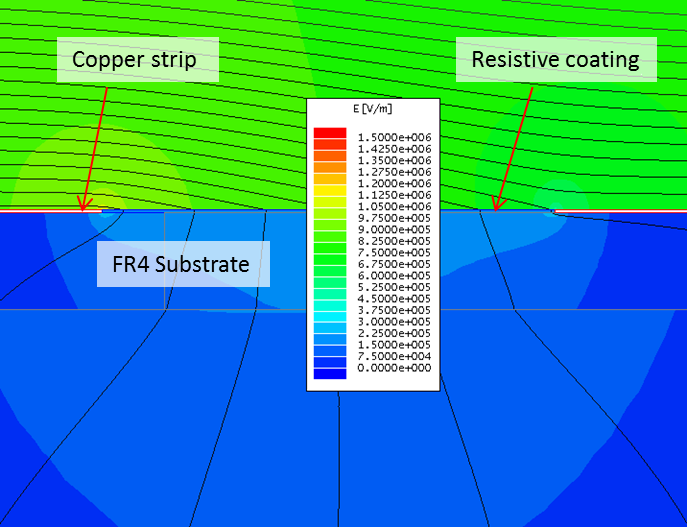
\includegraphics[width=4in]{tpc_fca_fea2.png}
\caption[FCA with resistive coating]{Electrostatic simulation of a field cage design that uses a layer of resistive coating between the conductive copper strips to eliminate the high field regions near the copper edges. }
\label{fig:tpc-field-cage-resistive-coating}
\end{figure}    


%%%%%%%%%%%%%%%%%%%%%%%%%%%%%%%%
\subsection{High Voltage Components}
\label{subsec:v5-tpc-hv}
   
The power supplies for the TPC cathode planes 
must be able to provide $-200$ kV at 1~mA current. The output voltage ripple 
must not introduce more than 10\% of the equivalent thermal noise from the front-end electronics. 
The power supplies must be programmable to trip (shutdown) 
their output at a certain current limit.  During power on and off, 
including output loss (for any reason), the voltage ramp rate at the 
feedthrough must be controllable to prevent 
damage to the in-vessel electronics through excess charge injection.

High-voltage feedthroughs must be able to withstand $-$250 kV 
at their center conductors in 1~atm air or argon gas environment when terminated in liquid argon.


\begin{figure}[htbp]
\centering
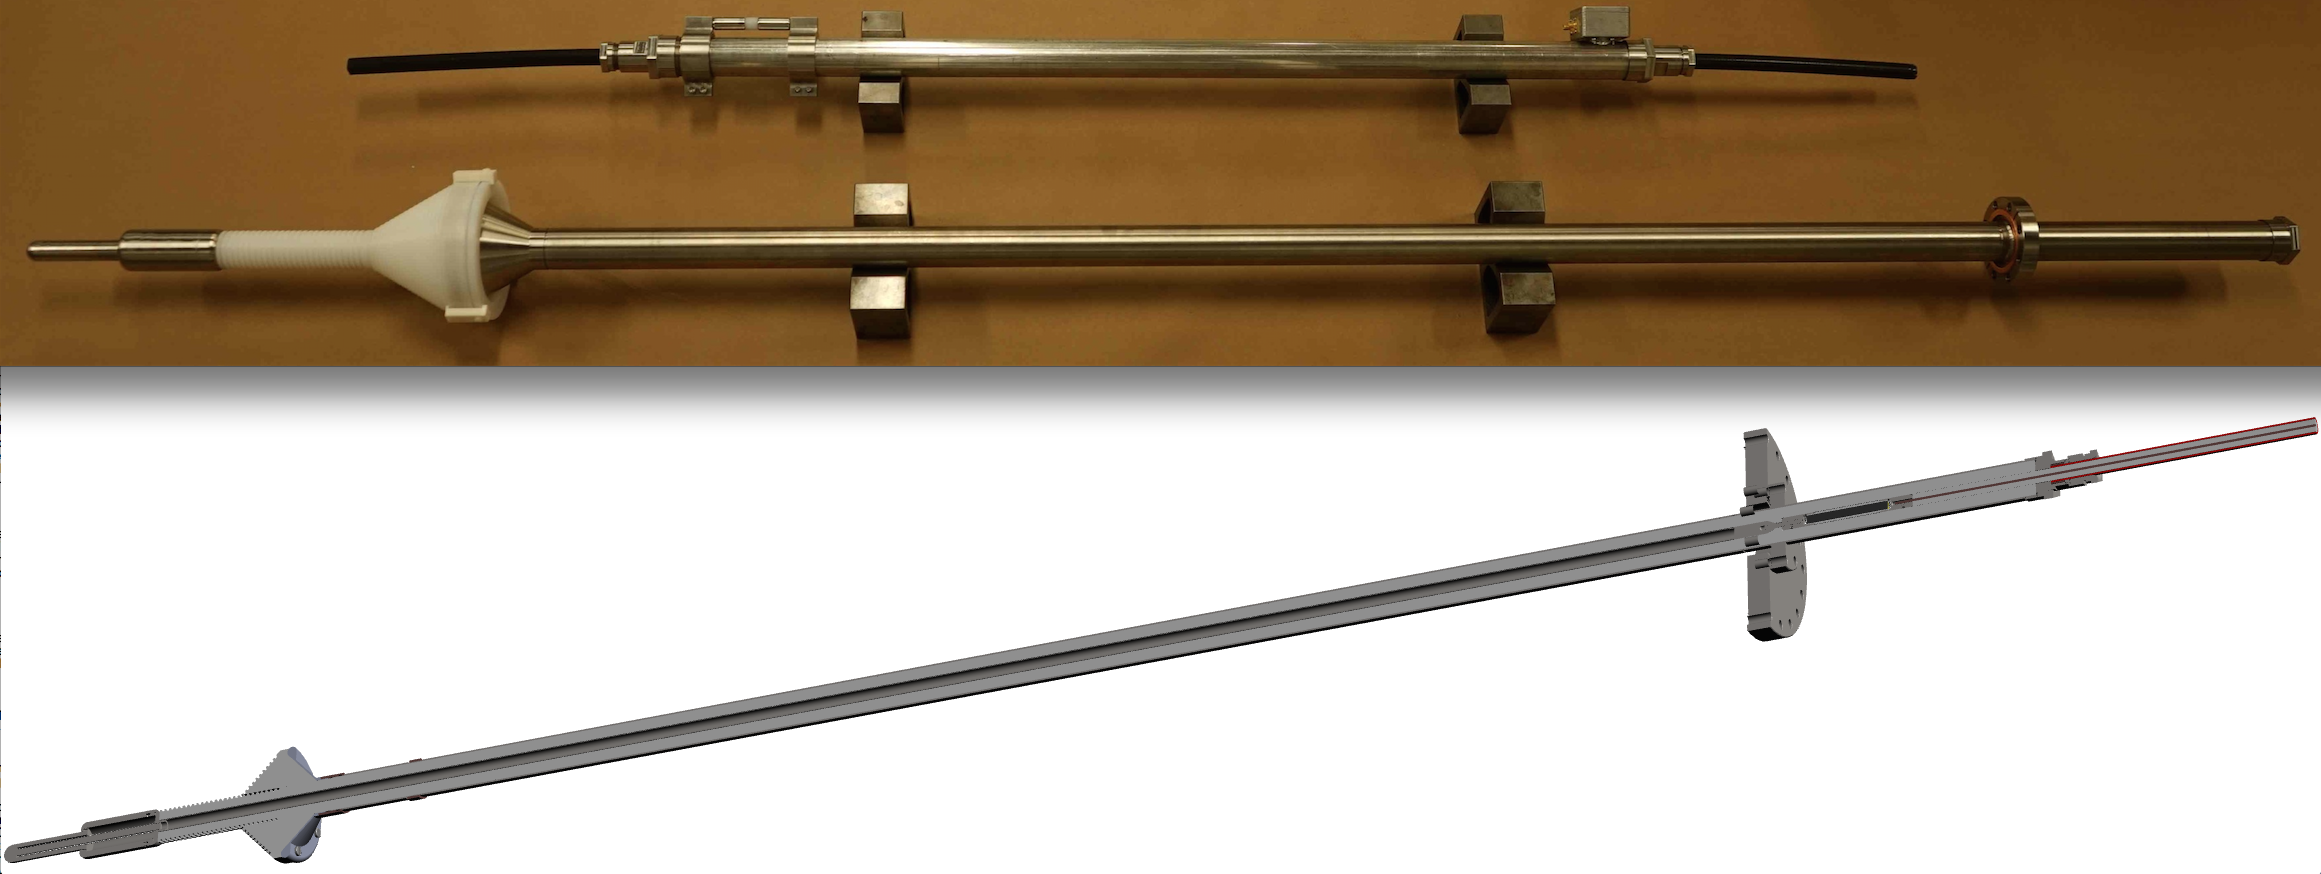
\includegraphics[width=\linewidth]{tpc_hv_feedthrough.png}
\caption[concept of new feedthrough]{Top: The high voltage feedthrough and filter developed by the UCLA 
group for the 35ton TPC.  It was tested up to 150 kV.  Bottom: a conceptual design of a new feedthrough for the LAr-FD.}
\label{fig:tpc-UCLA-feedthrough}
\end{figure}

The cathode planes are biased at $-$170~kV to provide the required 
500~V/cm drift field. At a minimum, three high-voltage power 
supplies, each connecting through their own feedthroughs, will be used. Each supply will
provide high voltage to one of the three rows of the cathode plane assemblies.

The current candidate for the high-voltage power supplies is 
the Heinzinger PNC{\it hp} series, which is used by the ICARUS 
experiment.  Additional filtering of the voltage ripples is done through the intrinsic HV cable capacitance 
and series resistors installed inside the filter box. Established techniques and practices will be implemented to eliminate 
micro-discharges and minimize unwanted energy transfer in case of an HV breakdown. 
  
To ensure safe and reliable operation, the feedthroughs will be 
tested at a much higher voltage than expected in
routine operation ($\sim$ 250 kV) in liquid argon. 
 The feedthroughs will be 
mounted on the ceiling of the cryostat, their cold ends reaching 
through the gas ullage space and submerging into the liquid argon. 
The center conductor on the cold side of a feedthrough will be 
insulated and shielded by a grounded shroud at least 50~cm below the 
surface of the liquid. Connections between the feedthroughs 
and the CPA rows are made through stainless-steel pipes in the 
liquid argon. Figure~\ref{fig:tpc-UCLA-feedthrough} shows an example 
of the feedthrough and filter box made by the UCLA group for the 35ton TPC, as well as the conceptual design of a feedthrough suitable for the LAr-FD TPCs.

%%%%%%%%%%%%%%%%%%%%%%%%%%%%%%%%
\section{TPC Assembly in the Cryostat}

\begin{figure}[htbp]
\centering
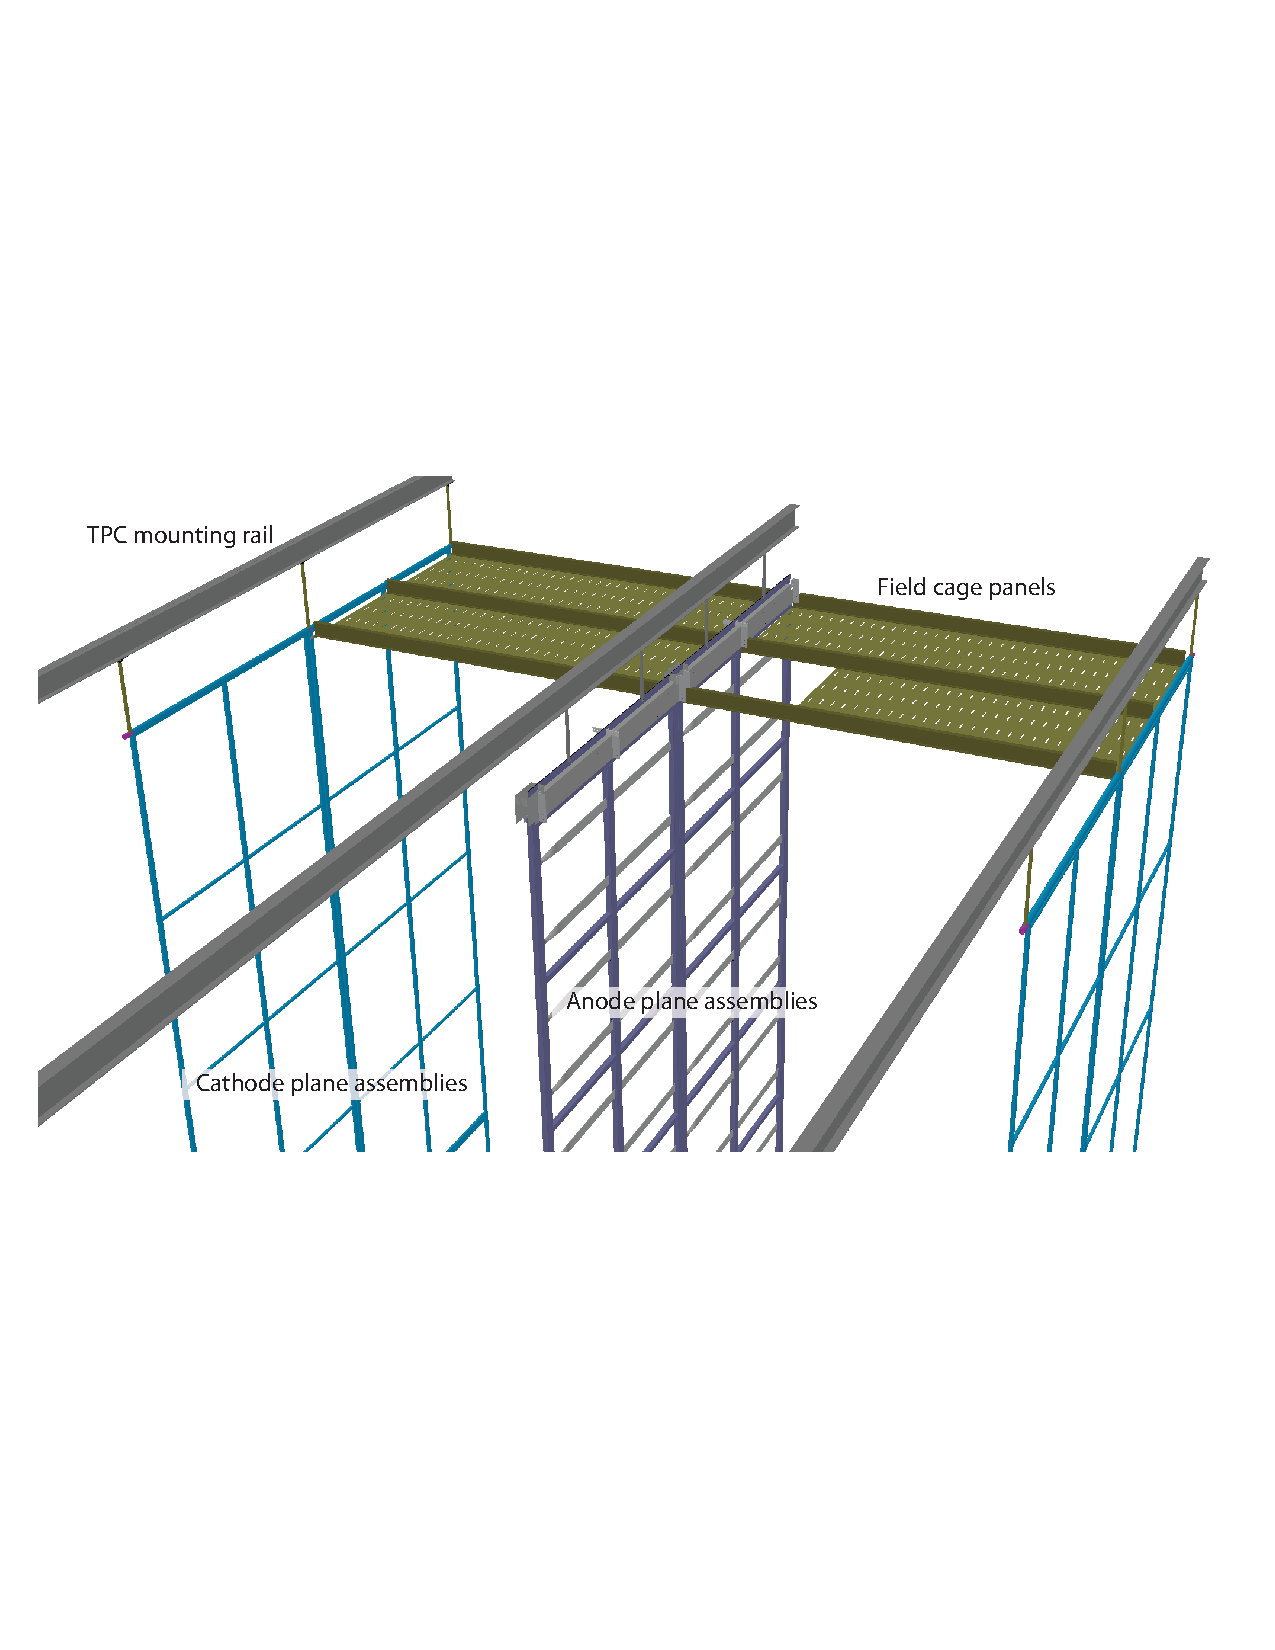
\includegraphics[width=\linewidth]{v5c3-tpc-partial-assembly}
\caption{A partial assembly of the TPC showing all major components}
\label{fig:tpc-partial-assembly}
\end{figure}

Figure~\ref{fig:tpc-partial-assembly} shows a partial assembly of a section of the TPC. The finished cryostat has five rows of anchor points distributed along the ceiling (not shown in the figure). A mounting rail is suspended through stainless-steel rods to each row of the anchor points. Under these five mounting rails, rows of CPAs and APAs are suspended in an interleaved fashion. Because the cathodes are at a high voltage, the CPAs are attached to their mounting rails through G10 rods. The distance between the facing anode and cathode is maintained by the pultruded fiberglass I-beams holding the FR4 sheets forming the field cage. The TPC installation procedure is discussed in  Chapter~\ref{ch:install}.




%%%%%%%%%%%%%%%%%%%%%%%%%%%%%%%%
\section{TPC Prototyping, Test and  Checkout}
\label{sec:v5-tpc-checkout}

%%%%%%%%%%%%%%%%
\subsection{TPC Prototyping}
\label{sec:v5-tpc-checkout-prototype}

Several prototype TPC modules were constructed during the design phase. The initial prototypes were fractional scale or partial models of the APA and CPA. The CPA prototype was used to evaluate field-shaping electrode attachment techniques. The APA prototype that was used to study the placement of the wire-wrapping boards and wire-support structures is shown in Fig~\ref{fig:tpc-apa-40percent}. It was also used to develop the prototype winding machines. The prototypes were subjected to numerous thermal cycles down to liquid-nitrogen temperature to test the integrity of the wire-to-board and board-to-frame bonds. 

\begin{figure}[htbp]
\centering
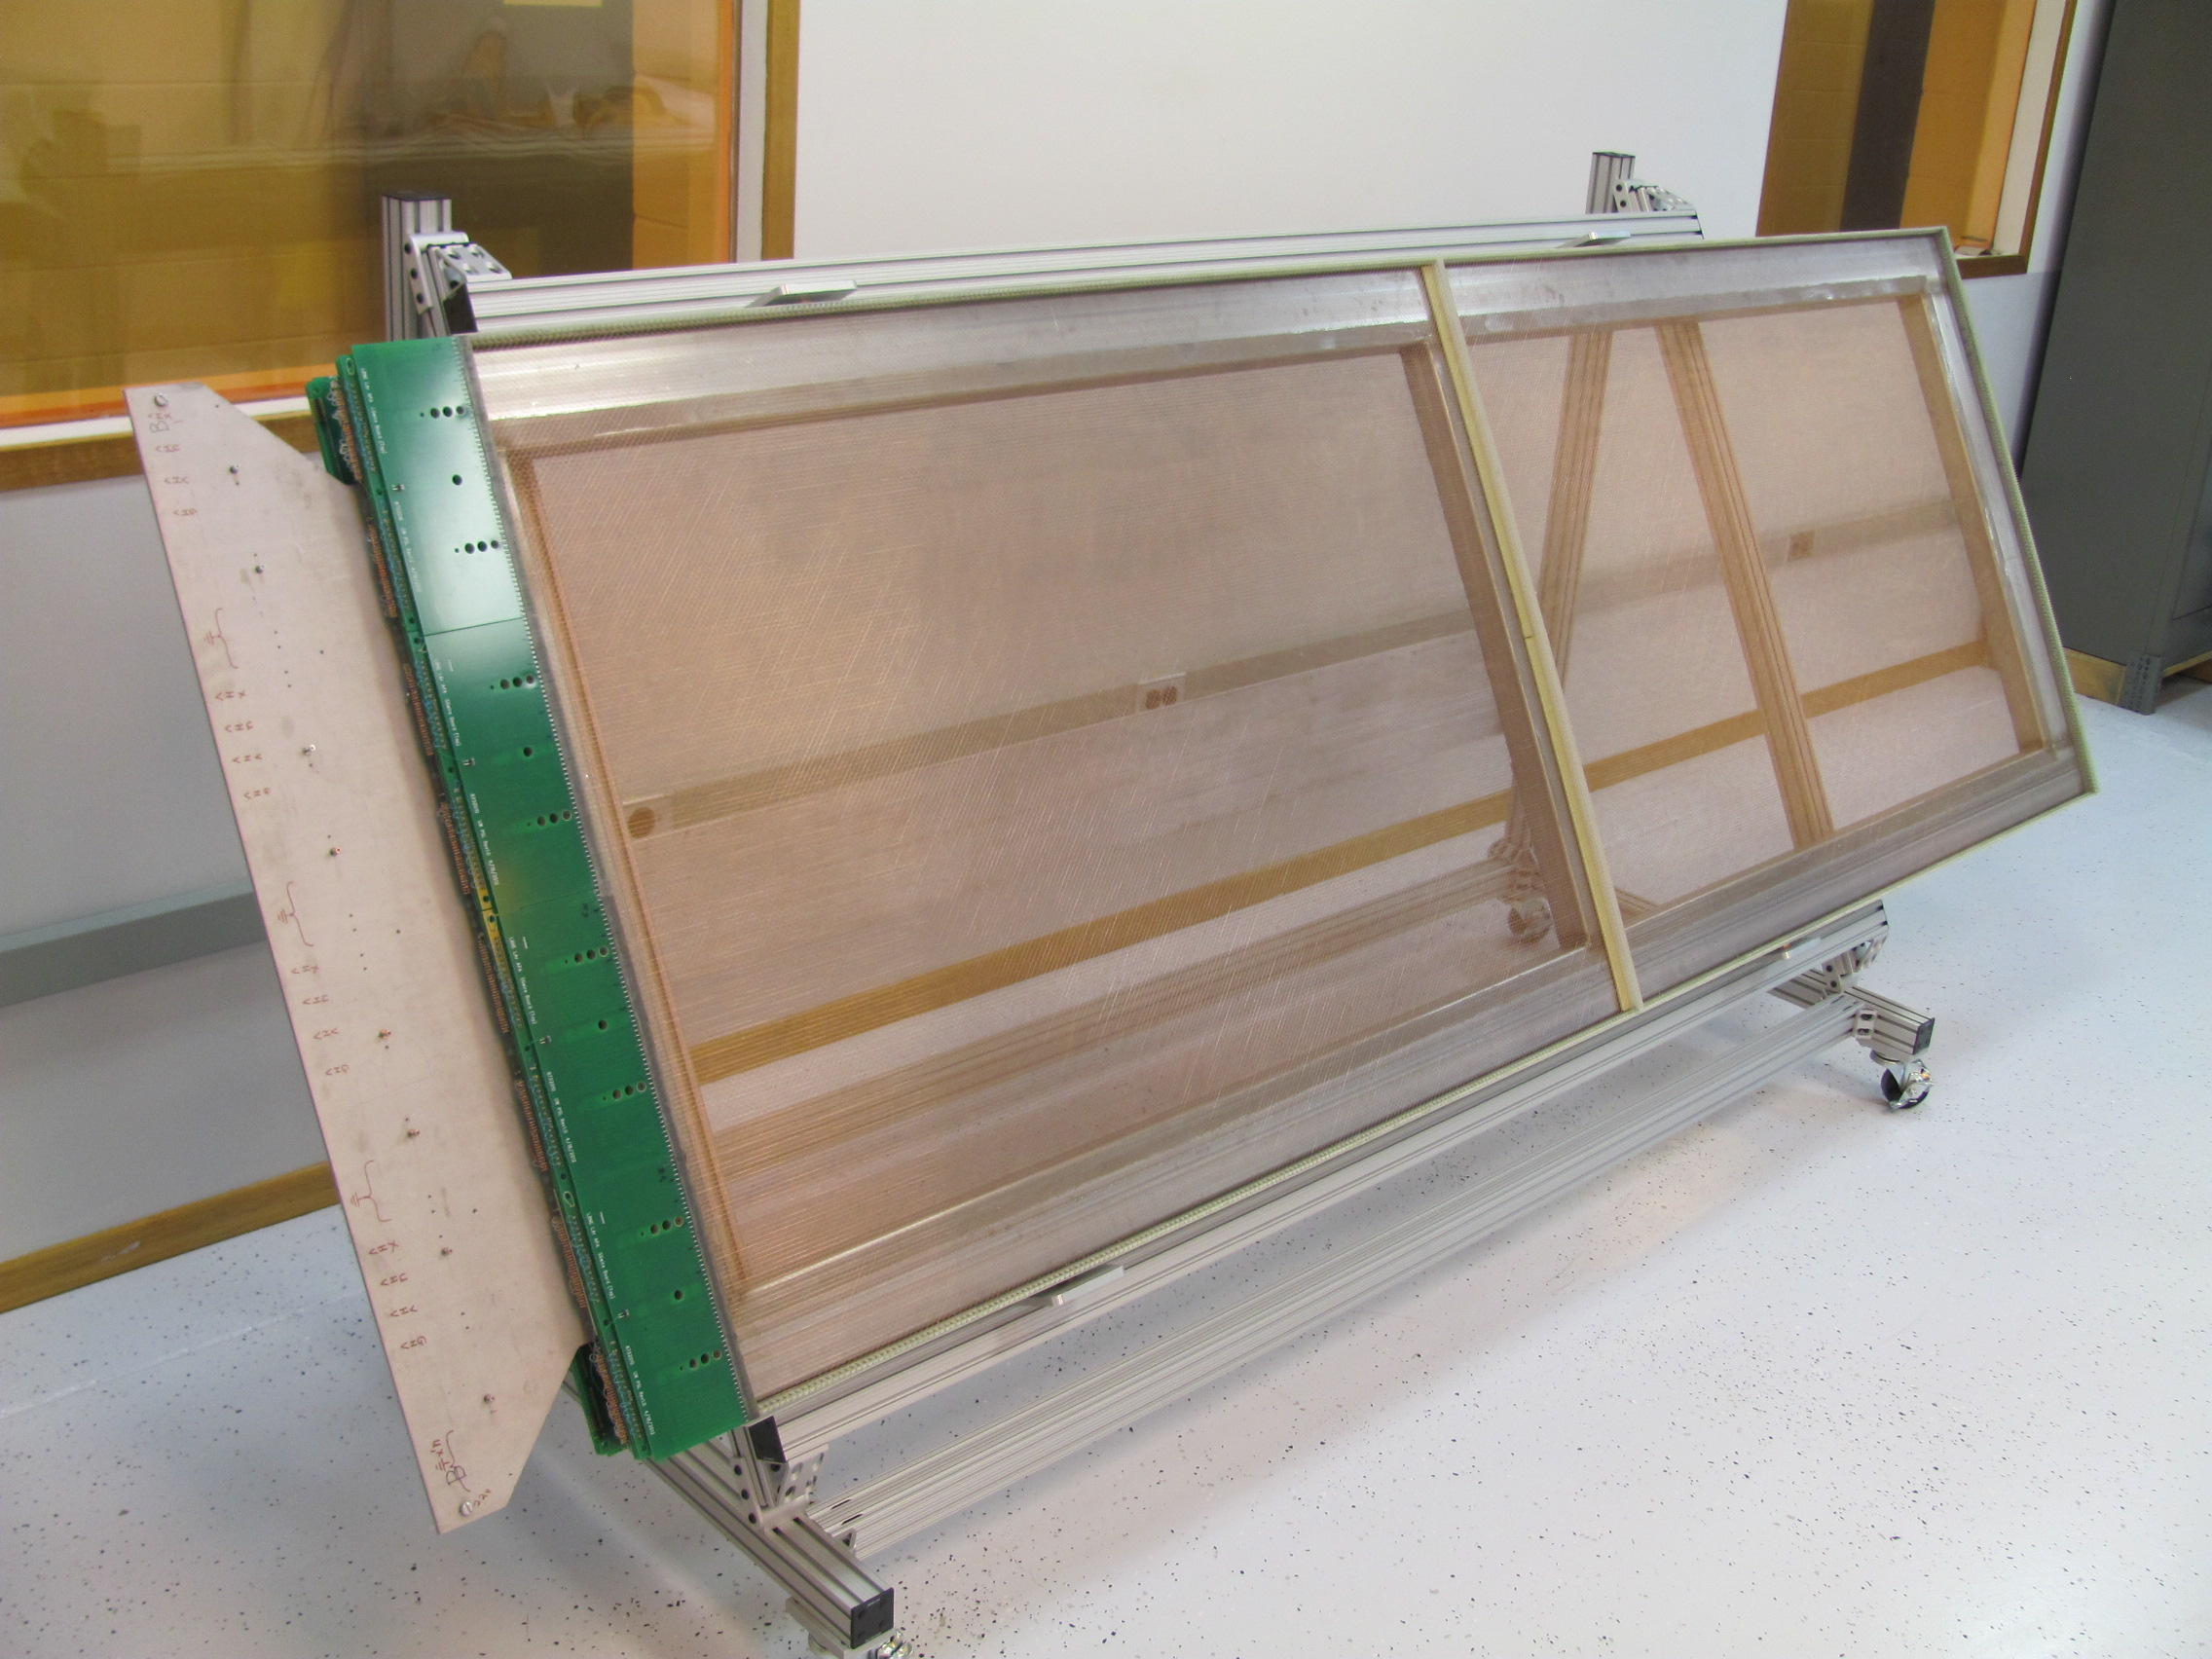
\includegraphics[width=\linewidth]{tpc_apa_40percent.jpg}
\caption{APA prototype that was used to study the support structure and wire wrapping}
\label{fig:tpc-apa-40percent}
\end{figure}


\begin{figure}[htbp]
\centering
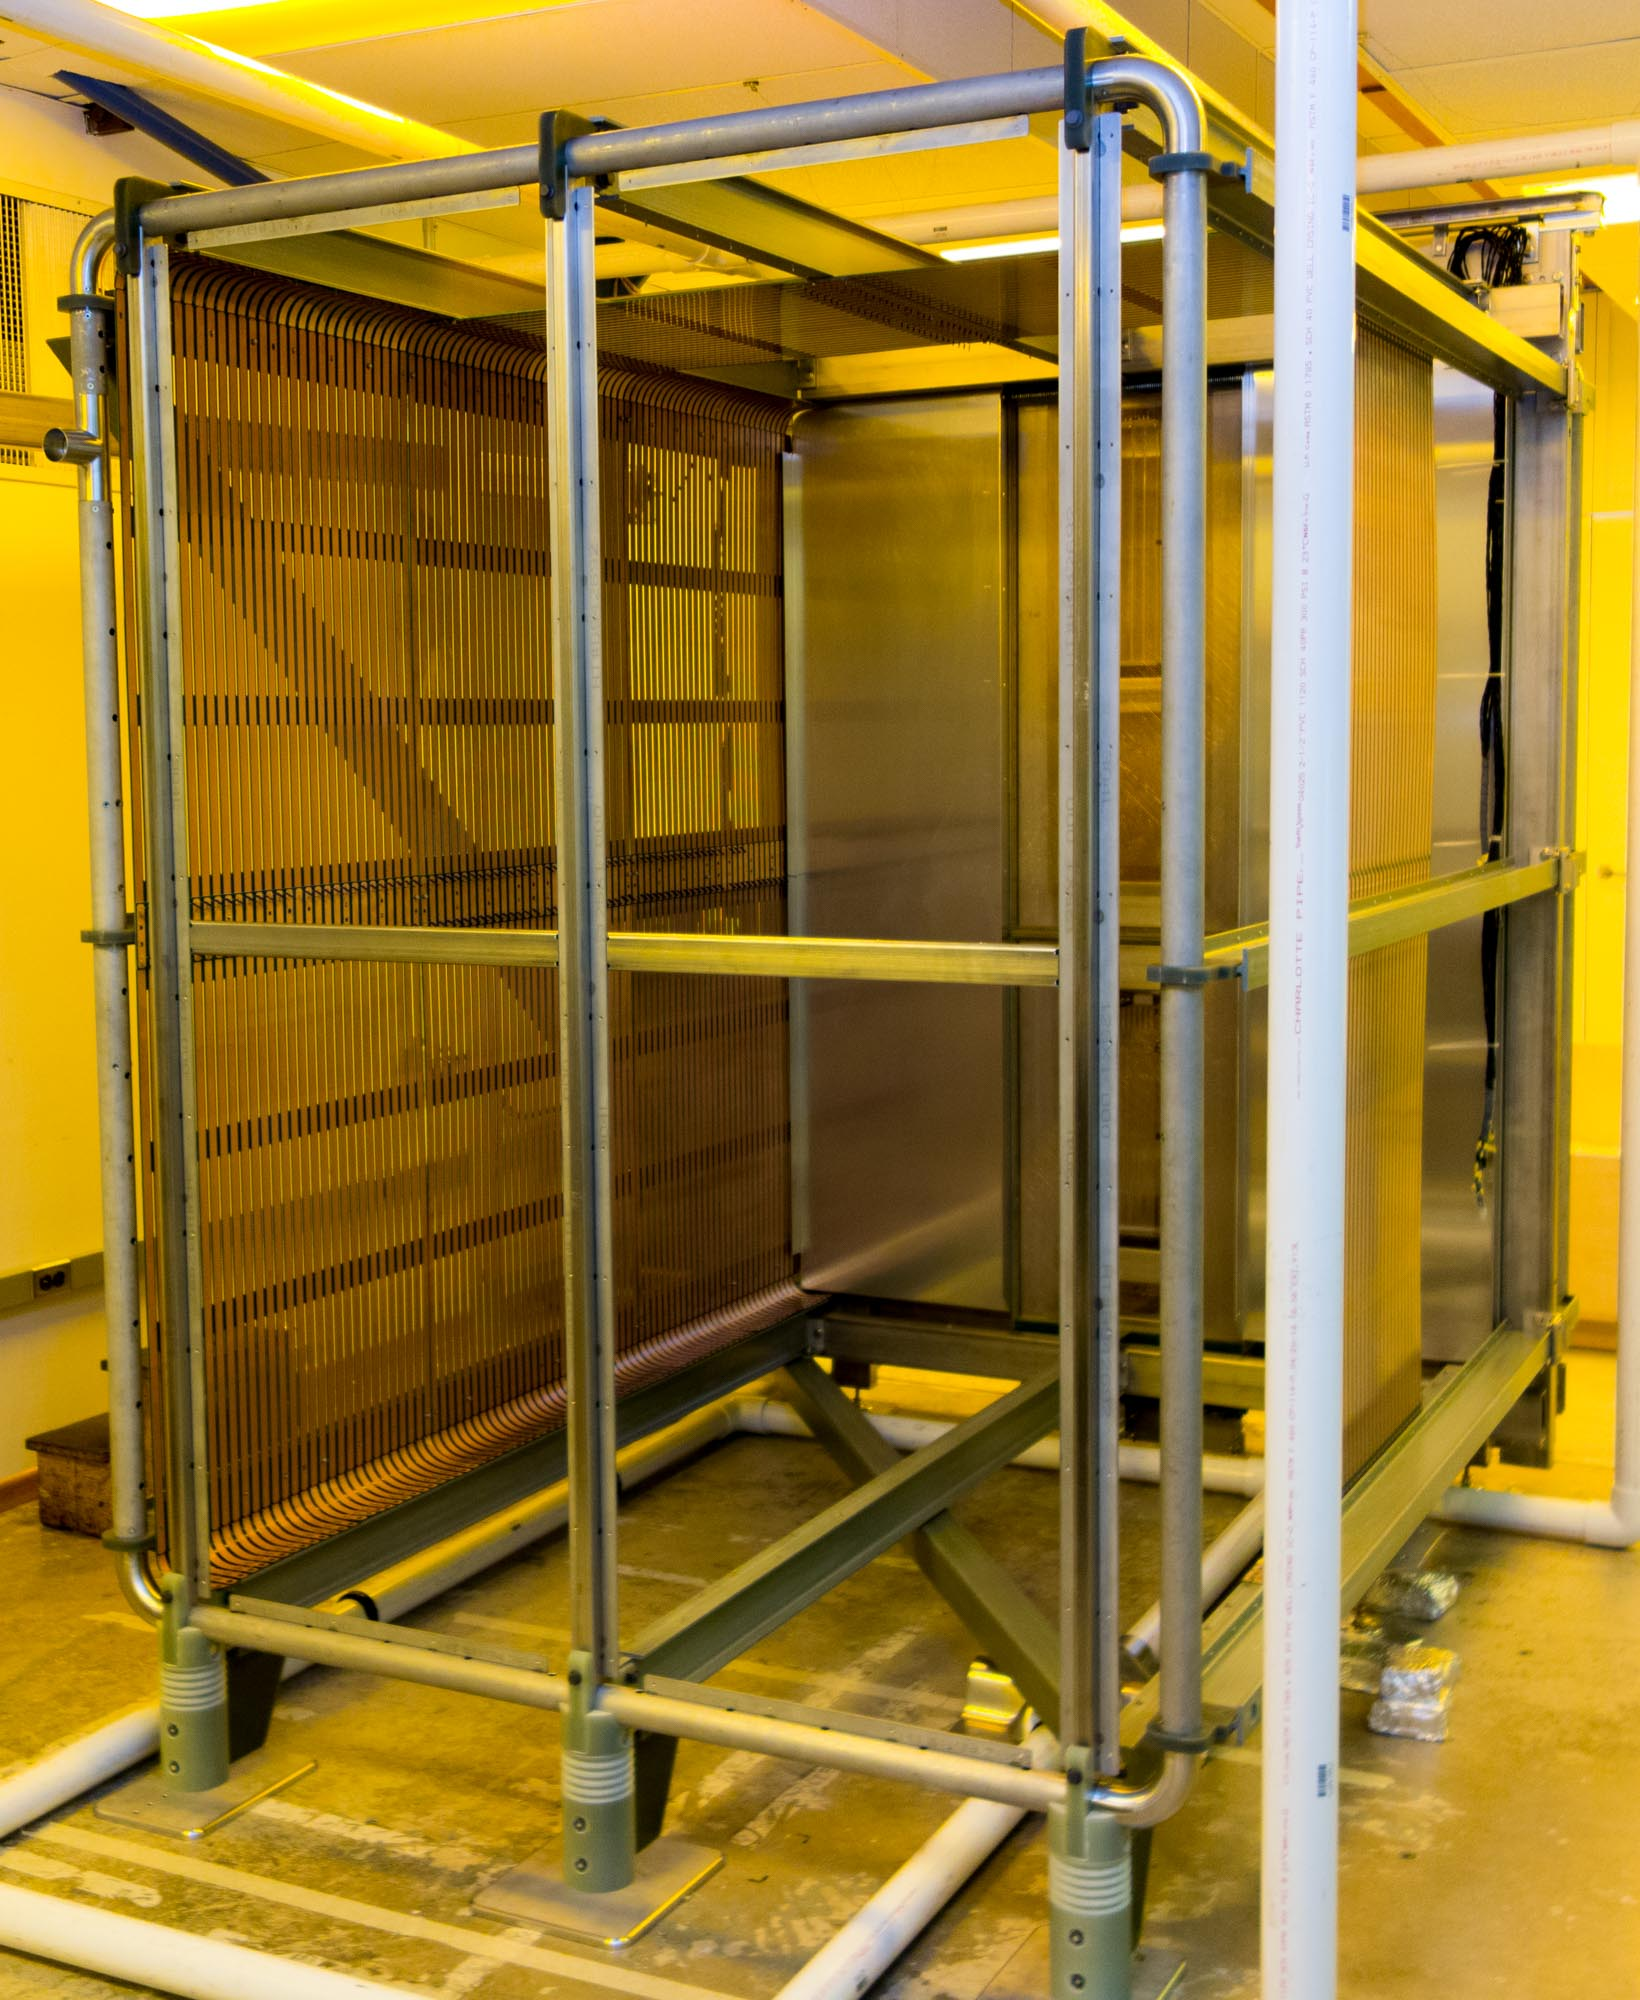
\includegraphics[width=\linewidth]{tpc_35ton_trial_assembly.jpg}
\caption{Trial assembly of the APAs, CPAs and field cage panels into the 35-t TPC.}
\label{fig:tpc-35ton-trial}
\end{figure}


The second set of prototypes are scale models of the APA and CPA. They are being used to validate the designs and to evaluate production procedures. Prototype front-end electronics boards for the scale APAs are currently being tested. Figure~\ref{fig:tpc-35ton-trial} shows the trial assembly of these functional prototypes into the TPC that will be installed in the 35 ton prototype cryostat. This TPC is expected to be operational in 2015.

A TPC prototype that is proposed to go into the CERN neutrino beamline requires three full-size APAs with fully instrumented readout electronics, six full-size CPAs, and complete field-cage coverage. The TPC will be constructed using identical APAs, CPAs and field-cage panels as designed for the LAr-FD. Additional features will be installed to ensure proper TPC operation given the half-height cryostat configuration. The construction and assembly of all TPC mechanical components will use the same materials and techniques as designed for LAr-FD, with the exception of a reduced degree of automation than will be used to wire APAs for the LAr-FD. 

A complete set of cold electronics will be installed on the APAs. The electronics components will closely resemble those designed for the LAr-FD. All key features of the LAr-FD electronics chain, including preamp, shaper, ADC, digital buffer, zero suppression and multiplexing will be implemented. Some electronics may be in prototype or functional-equivalent form.


%%%%%%%%%%%%%%%%
\subsection{Assembly Testing}
\label{sec:v5-tpc-checkout-test}

The components and the completed APAs will undergo thorough testings to ensure they meet the spec:
\begin{itemize}

\item The wire-carrier boards will be thermally cycled and HV stressed to check for excess leakage current.
\item The CR boards will be fully tested at the rated bias voltages of the capacitors at warm and cold.  Components showing excess leakage current at bias will be replaced.
\item The tension and electrical continuity of each wire will be 
measured after the plane of wires is bonded to the frame.
\item After the front-end electronics boards have been installed on 
the APA, an initial calibration of all electronic channels will be 
performed.  The electronic gains and noise levels of all channels will be 
recorded in a database.
\item A cool-down stress test will be performed on each completed 
APA in a liquid-nitrogen environment.  Electronic calibration on 
all channels will be performed while the APA is cold and again
after it is warmed up.  Significant differences in the cold and warm calibration 
results will be investigated and remediated.  
\end{itemize}

For the CPAs, a cool-down stress test will be performed on each completed 
CPA in a LN$_2$ environment to verify its flatness at cryogenic temperature. If resistive surfaces are used on the cathode, its contact resistivity to the outer metal frame at warm and cold will be verified to be within spec. 

For the field cages,  the resistance will be measured along each copper strip,  
and between strip pairs.  The resistance between two 
strips should exceed 50 G$\Omega$, without the resistive divider.  All resistor will be thermal cycled before installing on the divider.  Any resistor with resistance beyond spec in the cold will be rejected. All varistor will be also be thermal cycled, and their leakage current at nominal operating voltage as well as their clamping voltages at cold verified.  High voltage tests may be performed on all field cage assembles to identify manufacturing defects on the surfaces. 

%%%%%%%%%%%%%%%%
\subsection{Checkout } 
\label{sec:v5-tpc-checkout-checkout}

After passing the tests at the assembly level, the APAs will be put into storage, and later transported to the LBNE Far Site. Prior to installation, another round of electronic calibration will be performed on the APAs to validate their acceptable status. 

During installation, the DAQ system will be running continuously. As soon as each stack of APAs is connected to the pre-routed cables, a suite of calibration runs will be performed to validate that all connections have been made properly. Repair or replacement at this stage will still be straightforward. 

After the entire TPC is assembled, a system-wide calibration will be performed at room temperature and again at cryogenic temperature in argon gas. Repair or replacement would require partial disassembly of the TPC and should be avoided unless absolutely necessary. 

The responsibility and authority for the design, installation and use of the detector quiet-power distribution and detector-grounding system is held by the subproject electrical engineer. This engineer has oversight responsibility for all electrical and electronics design and installation tasks, including all attachments to the detector that create an electrical connection. 



